\chapter{The X.509 standard and PKI}
We will now discuss the X.509 standard and Public Key Infrastructure 
(PKI), which is widelly adopted for public key certification.
\section{Public-key certificate (PKC)}
Lets begin with a definition:
\begin{boxH}
  A \textbf{public-key certificate} is a \textbf{data structure} to securely
  bind a public key to some attributes.
\end{boxH}
A PKC is said to "securely bind" a public key to some attributes
because it is signed by a trusted entity, the \textbf{Certification
Authority}, but other techniques for certification exists (e.g.
blockchain, direct trust and personal signature).\\
The attributes in the certificate are those employed in the
transaction being protected by the PKC, which are difficult to decide
a-priori without knowing the context: for example one attribute could
be an email address associated with the entity, which may not be valid
for all the transactions.\\
PKC are most important to achieve \textbf{non-repudiation}, many
certificates have legal value, and \textbf{digital signature} in a
secure way.\\
\begin{boxH}
  Keep in mind that a PKC is the complement of a corresponding
  \textbf{personal private key}, which is kept secret by the entity.
\end{boxH}
Which means that if the private key is compromised, the PKC is 
compromised as well.
\subsection{Key Generation in Public Key Cryptography (PKC)}

Key generation in public key cryptography (PKC) involves complex
algorithms and often relies on random number generators (RNGs) to
ensure strong, unpredictable keys. Once a key is generated, the
private key must be securely protected in various contexts:

\begin{itemize}
  \item \textbf{Storage}: The private key needs to be securely
    stored to prevent unauthorized access.
  \item \textbf{Usage}: The private key must also be protected when
    being used, as it could be exposed during operations in the CPU as
    it is used in clear text.
  \item \textbf{Software Application}: In software environments
    (e.g., web browsers), the trustworthiness of the computing
    platform must be considered, as it may be vulnerable to malware
    or weak implementations. This is true both for the context of
    key generation and use.
  \item \textbf{Dedicated Hardware}: Storing and using keys in
    dedicated hardware, such as a smart card, offers enhanced
    protection but comes with limitations in terms of algorithm
    updates or vulnerability patching( which may be difficult or
    even impossible). For example many old smart cards use 1024-bit 
    RSA keys, which are considered insecure today.
  \item \textbf{Key Injection}: Keys may be generated in software
    and injected into hardware devices, a process that can be useful
    for key recovery, but should be restricted to encryption keys to
    maintain security and ensure non repudiation. This is most
    important for the private key. 
\end{itemize}

PKC key management requires careful consideration of both security and
operational challenges, especially when dealing with long-term
security mechanisms.

\subsection{Certification architecture}

In Public Key Infrastructure (PKI), several key entities are
responsible for managing the lifecycle of Public Key Certificates
(PKCs):

\begin{itemize}
  \item \textbf{Certification Authority (CA)}: The CA is responsible
    for generating and revoking PKCs. It also publishes PKCs and
    maintains information about their status, such as whether they
    are valid or revoked, or even suspended.
  \item \textbf{Registration Authority (RA)}: The RA plays a
    critical role in verifying the claimed identity and attributes
    of a certificate requestor. It authorizes the issuance or
    revocation of PKCs but does not generate them itself.
  \item \textbf{Validation Authority (VA)}: The VA provides services
    that allow third parties to verify the validity status of a PKC,
    because some responsibilities or the RA may be delegated to it.
    This may involve downloading Certificate Revocation Lists (CRLs)
    or querying an Online Certificate Status Protocol (OCSP)
    responder to check the certificate's status in real-time.
  \item \textbf{Revocation Authority}: Although not an official
    term, this role may be assigned to either the RA or CA. The
    revocation authority is delegated to revoke certificates, often
    on a more urgent basis than their issuance (they are available
    most of the time), ensuring that compromised or invalid
    certificates are promptly rendered unusable.
\end{itemize}

These entities work together to ensure the security and
trustworthiness of PKC-based systems by handling key tasks such as
certificate issuance, verification, and revocation.

\subsection{Certificate generation}
The general
When an actor want to generate a certificate, it must first generate a 
key pair (public and private key). The private key is stored locally
and protected(encrypted) as good as possible, while the public key 
is sent to the CA with some attributes that help identify the actor.\\
The CA requires that the attributes are both correct and are
associated actually with the entity that is in control of the private
key, which requires authentication of the actor. For that purpose, if
the entity is a human it is usually required to go physically to the 
CA, even if in some cases a video call may be enough, with the 
requirement of showing a valid ID.\\
The Registration Authority will verify the attributes and the 
identity of the actor, and if everything is correct, it will send a 
message to the CA to generate the certificate.\\
At this point the CA generates the certificate, signs it with its 
private key and sends it back to the actor while also storing it in 
its repository.\\
As you may noticed, the verification is only on the attributes, and
not of the possession of the private key, which will be discussed
later.

\begin{figure}[h]
  \centering
  \includegraphics[width=0.8\textwidth]{img/x509 certificate
  generation.png}
  \caption{Certificate generation}
\end{figure}

\subsubsection{Another certificate generation architecture}

In addition to what just discussed, alternative architectures for
certificate generation exist:

\begin{itemize}
  \item \textbf{Key Pair Generation by RA}: In some architectures, the
    Registration Authority (RA) generates the key pair on behalf of
    the user, obtains the Public Key Certificate (PKC), and securely
    distributes the key pair and certificate to the user via a
    secure device, such as a smart card. This approach is often used
    in large companies where the employees are already known to the
    organization.

  \item \textbf{User Authentication via Code}: Another common method
    involves the user visiting the RA to obtain a code that can be
    used to authenticate their certificate request to the
    Certification Authority (CA). The code is typically calculated
    as a Message Authentication Code (MAC) using the shared secret
    key between the RA and CA:

    \[
      \text{code} = \text{MAC}(K, ID)
    \]

    where \(K\) is a shared secret key between the RA and CA, and
    \(ID\) is the user's identity. The user then submits this code to
    the CA to validate the certificate request.
\end{itemize}

These alternative methods provide flexibility for organizations with
different security needs, allowing for centralized key generation and
secure certificate distribution.

\section{X.509 certificates}

X.509 is an ITU-T (international telecommunication unit body) standard
that defines the format of public key certificates used to verify the
identity of a key owner in cryptographic systems. X509 was developed
as a certification technology to protect the x500 directory service,
and has undergone several versions:

\begin{itemize}
  \item \textbf{v1 (1988)}: The initial version of the standard.
  \item \textbf{v2 (1993)}: A minor update with small improvements.
  \item \textbf{v3 (1996)}: Added extensions and introduced version
    1 of the attribute certificate.
  \item \textbf{v3 (2001)}: Further enhancements, including version
    2 of the attribute certificate, which are not used anymore.
\end{itemize}

X.509 is part of the larger X.500 standard for directory services,
often referred to as "white pages," which are used for managing
information about entities in a structured way(directory services).
X.509 provides a solution to the problem of securely identifying the
owner of a cryptographic key.

The certificates and their structures are defined using \textbf{ASN.1}
(Abstract Syntax Notation One), a standard interface for defining data
structures exchanged in networking environments in a neutral and 
platform-independent way. 

\subsection{PKC Scope}
A Public Key Certificate (PKC) contains information that uniquely
associates a cryptographic key with an entity. This binding between
the key and the entity is ensured by a \textbf{Trusted Third Party
(TTP)}, typically referred to as a Certification Authority (CA), which
digitally signs each certificate to guarantee its authenticity.\\

The liability associated with a PKC may be restricted to specific
applications or purposes, as outlined in the CA's certification
policy. This policy defines the intended usage and limits the scope of
the certificate, ensuring it is applied within the proper legal and
technical contexts.

\subsection{Certificate Policy (CP) and Certification Practice
Statement (CPS)}

According to RFC-3647, "Internet X.509 Public Key Infrastructure
Certificate Policy and Certification Practices Framework," both the
Certificate Policy (CP) and Certification Practice Statement (CPS)
play key roles in defining the use and management of Public Key
Certificates (PKCs):

\begin{itemize}
  \item \textbf{Certificate Policy (CP)}: A CP is a named set of rules
    that defines the applicability of a PKC to a specific community
    or class of applications with common security requirements. It
    establishes the minimum requirements for the issuance and
    management of certificates and can be followed by multiple
    Certification Authorities (CAs). For example, a government CP
    may apply to all certification providers issuing certificates
    for official use.

  \item \textbf{Certification Practice Statement (CPS)}: A CPS outlines
    the specific practices that a CA follows when issuing PKCs.
    While a CP specifies the general rules, the CPS provides
    detailed implementation procedures. Each CA develops its own
    CPS, which is tailored to its operations and describes how it
    meets the requirements set forth in the CP.
\end{itemize}

\subsection{X.500 Directory Service}

The X.500 directory service was the first system to use X.509v1
certificates. It aimed to manage information about people and entities
in a network. However, this early setup had three big issues:

\begin{itemize}
  \item \textbf{No Guarantees on the CA's Quality}: There weren't
    clear rules or policies to ensure that Certification Authorities
    (CAs) were reliable or trustworthy. People just had to trust the
    CA, which caused concern over the security of the certificates.

  \item \textbf{Lack of a proper X.500 Infrastructure}: Even though
    certificates were supposed to be stored in X.500 directories, the
    infrastructure to do this was never fully implemented worldwide.
    This made it tough to access certificates when needed.

  \item \textbf{Hard to Establish Certification Paths}: It was
    difficult to connect two users with certificates issued by
    different CAs because the relationships between CAs weren’t
    well-defined. With each CA running its own domain, figuring out
    how to establish a secure connection between users from different
    domains was tricky.
\end{itemize}

These issues slowed down the adoption of X.500 and made it clear that
better systems were needed for managing certificates.

\subsubsection{Fixing X.509v1 Problems}

To solve these problems, X.509v1 was updated with a couple of key
changes:

\begin{itemize}
  \item \textbf{Move the semantics Outside the Certificate}: Instead of
    relying on the certificate itself to define its semantics, they
    decided to put that responsibility on the application or some
    external system. This approach was used in things like RFC-1422
    (PEM), where the application takes care of interpreting the
    certificate.

  \item \textbf{Make Certificates More Flexible}: The original X.509v1
    certificates were pretty limited: they only had an identifier and a
    key. With X.509v3, they added more fields and options to make
    certificates more flexible and useful for a variety of purposes.
    This allowed them to handle a wider range of security scenarios.
\end{itemize}

These updates helped fix the early issues and set the stage for
broader adoption of the improved X.509v3 certificates.

\subsection{RFC-1422}
RFC-1422 tried to fix some of the problems with the early X.500
systems by proposing a worldwide certification hierarchy. The plan was
to have one main CA at the top: the \textbf{IPRA} (Internet Policy
Registration Authority). This CA would be responsible for setting the
rules and policies for all other CAs in the system, ensuring that
everyone followed the same security practices.\\
Instead of directly issuing certificates to lower-level CAs, the IPRA
would issue certificates to \textbf{Policy Certification Authorities
(PCAs)}.\\
The IPRA oversaw the entire structure and laid out specific
roles for different types of Certification Authorities (CAs) to manage
and enforce certificate policies:

\begin{itemize}
  \item \textbf{Policy Certification Authority (PCA)}: PCAs were
    responsible for setting and enforcing the policies that governed
    how certificates were issued. They made sure that the CAs under
    them followed the right security practices.
  
  \item \textbf{Name Subordination}: CAs had to issue certificates
    within a defined part of the naming structure, ensuring a
    consistent and organized system. For example:
  \begin{itemize}
      \item \textbf{CA n.1}: C=IT (country-level CA for Italy)
      \item \textbf{CA n.2}: C=IT, O=Politecnico di Torino (CA for an
        organization within Italy)
  \end{itemize}
\end{itemize}


 However, this system wasn’t without flaws—it
was still based on geographic hierarchies, which didn’t always match
the needs of modern, global organizations.

The IPRA was established, and four PCAs were created under it. One of
these PCAs was designated as \textbf{high assurance}, meaning it had
to carry out stricter checks before issuing certificates. For
instance, BBN, a company heavily involved with the U.S. military,
might require things like fingerprints or even DNA tests to verify
identities.

In contrast, \textbf{mid-level assurance} certificates, like those
issued by universities such as MIT, required less rigorous
checks—maybe just showing a passport. MIT could even set up its own
subordinate CAs, like one for the Laboratory for Computer Science, to
handle its internal certificate needs.

What’s interesting is how different cultural practices shaped the
certification process. In the U.S., where people don’t generally carry
ID cards, \textbf{residential certification authorities} were used. If
you wanted to open a bank account, for example, you might have to show
an electricity bill to prove your address. While this seems strange in
countries with formal ID systems, in the U.S., it was a necessity.

Finally, there were \textbf{persona certificates}, which allowed for
anonymous certificates. These were for users who didn’t want to reveal
their identity but still needed secure communications. For example,
you could be “anonymous user number 95.” Even though no one knew who
you were, the security of your communication was still guaranteed.

\begin{figure}[h]
  \centering
  \includegraphics[width=0.8\textwidth]{img/x509 internet per
  hierarchy.png}

  \caption{Internet PEM hierarchy (RFC-1422)}
\end{figure}

Unfortunately, this system was a complete failure for several reasons:

\begin{itemize}
  \item The hierarchical structure severely limited flexibility, much
    like the issues we saw with X.500. For international companies,
    this rigid hierarchy simply didn't work.

  \item Name subordination imposed additional restrictions. You
    couldn't just assign any name—you had to follow the strict
    hierarchy, which wasn't always practical.

  \item The use of the PCA concept lacked flexibility, especially in
    commercial settings. Instead of automating the process, a human
    operator was needed to check if the requester was following the
    policy. This made the system cumbersome and inefficient for
    businesses.

  \item Lastly, the biggest issue was trust. Where would the IPRA be
    placed? Naturally, the U.S. wanted it, but other countries, like
    Russia, China, or even Japan, wanted control as well. No one
    trusted a single country to sit at the top of the hierarchy,
    fearing the possibility of a fake hierarchy being created. As a
    result, the experiment collapsed. It briefly existed, primarily
    used by the United States, but it never gained global traction.
\end{itemize}

\section{X.509 Version 3}

X.509 Version 3 is a standard that was finalized in June 1996 through
a collaborative effort between ISO, ITU, and the IETF, with the goal
of making certificates suitable for internet applications. This
version consolidated all the necessary updates to certificates and
Certificate Revocation Lists (CRLs) into a single document. Earlier
versions of X.509 (v1 and v2) relied on external semantics, such as
the failed attempt with the Internet PEM hierarchy, which proved
unsuccessful. X.509v3 addressed these shortcomings by ensuring
certificates would be useful for internet applications, particularly
as OSI applications became mostly obsolete.\\
Key features of X.509 Version 3 include:

\begin{itemize}
  \item \textbf{Types of Extensions}:
    \begin{itemize}
      \item \textbf{Public Extensions}: These are defined by the
        standard and made publicly available for anyone to use.
        Because they are standardized, any system or application
        should be able to understand and process them.
      \item \textbf{Private Extensions}: These are tailored to
        specific user communities and are not publicly available. If a
        system does not understand a private extension, it will treat
        it as a binary blob and discard it. Private extensions are
        crucial for certain organizations that require custom
        functionality.
    \end{itemize}
    
    The introduction of extensions is a major improvement in X.509v3,
    adding flexibility without changing the fundamental structure of
    the certificate (which remains the same as in X.509v1). Extensions
    are contained within a small field but open up a wide range of
    possibilities. Public extensions ensure standard compatibility,
    while private extensions allow customization specific to
    organizations.

  \item \textbf{Certificate Profile}: This refers to a set of
    extensions tailored for a specific purpose or application,
    ensuring that certificates meet particular requirements. For
    example, RFC 5280, titled "Internet X.509 Public Key
    Infrastructure Certificate and Certificate Revocation List (CRL)
    Profile," provides guidelines on how X.509 certificates and CRLs
    should be structured for protecting internet applications.
    Certificate profiles are important because they dictate how
    certificates should be used for different scenarios, ensuring
    consistency and security.
\end{itemize}


\subsection{Base syntax}

The base syntax of an X.509 certificate is defined as follows:

\begin{verbatim}
Certificate ::= SEQUENCE {
    signatureAlgorithm AlgorithmIdentifier,
    tbsCertificate TBSCertificate,
    signatureValue BIT STRING
}

TBSCertificate ::= SEQUENCE {
    version [0] Version DEFAULT v1,
    serialNumber CertificateSerialNumber,
    signature AlgorithmIdentifier,
    issuer Name,
    validity Validity,
    subject Name,
    subjectPublicKeyInfo SubjectPublicKeyInfo,
    issuerUniqueID [1] IMPLICIT UniqueIdentifier OPTIONAL,
        -- if present, version must be v2 or v3
    subjectUniqueID [2] IMPLICIT UniqueIdentifier OPTIONAL,
        -- if present, version must be v2 or v3
    extensions [3] Extensions OPTIONAL
        -- if present, version must be v3
}
\end{verbatim}

This abstract notation outlines the basic structure of the
certificate. The \texttt{Certificate} is defined as a sequence, which
is a data structure that includes several fields. The first field,
\texttt{signatureAlgorithm}, is the algorithm identifier used by the
Certificate Authority (CA) to sign the certificate. 

Next, the \texttt{tbsCertificate} (to be signed certificate) is of
type \texttt{TBSCertificate}, which contains the main information that
needs to be signed. Finally, the \texttt{signatureValue} is a bit
string that holds the actual signature.

The \texttt{TBSCertificate} is again defined as a sequence, starting
with the \texttt{version} field, which begins numbering with zero,
indicating version 1. For version 3, this field has a value of two.
Following that, we have the \texttt{serialNumber} of the certificate
and the \texttt{signature} algorithm identifier. 

You may wonder why the signature algorithm appears twice—once
externally and once within the \texttt{TBSCertificate}. The external
algorithm identifier is crucial for verifying the signature; without
knowing the algorithm, you cannot validate the signature value. Having
it specified internally helps ensure that the signature algorithm used
for verification matches the algorithm used for signing. If they
differ, it's a red flag, indicating that the certificate should not be
trusted.

The \texttt{issuer} field identifies the certification authority by
name, and the \texttt{validity} field specifies the validity period of
the certificate. The \texttt{subject} is identified by its name, and
the \texttt{subjectPublicKeyInfo} field contains both the algorithm
and the actual public key of the subject.

In addition, versions 2 and 3 introduce optional unique identifiers
for both the issuer and subject, though these identifiers are rarely
used today. Finally, the \texttt{extensions} field, which is optional,
must be present for certificates of version 3, as earlier versions do
not support extensions.


\subsection{Critical Extensions}

In the context of X.509 certificates, extensions can be classified as
critical or non-critical, each affecting the certificate verification
process differently:

\begin{itemize}
  \item \textbf{Critical Extensions}: If a certificate contains an
    unrecognized critical extension, it \textbf{MUST} be rejected
    during the verification process. This ensures that any essential
    information required for proper validation is recognized and
    handled appropriately.

  \item \textbf{Non-Critical Extensions}: Conversely, a non-critical
    extension \textbf{MAY} be ignored if it is unrecognized. This
    allows flexibility in certificate processing, as non-critical
    information does not impede the overall verification of the
    certificate.
\end{itemize}

The responsibility for handling these extensions lies entirely with
the entity performing the verification, referred to as the
\textbf{Relying Party (RP)}. The RP must implement logic to correctly
interpret and respond to both critical and non-critical extensions in
accordance with their definitions.

\subsection{Public Extensions}

X.509 version 3 defines four classes of public extensions that enhance
the functionality and applicability of certificates:

\begin{itemize}
  \item \textbf{Key and Policy Information}: Extensions in this
    class provide additional information regarding the key usage and
    policies applicable to the certificate, guiding how the key
    should be used within specific contexts.

  \item \textbf{Certificate Subject and Certificate Issuer
    Attributes}: These extensions include attributes related to both
    the subject of the certificate (the entity that the certificate
    represents) and the issuer (the Certification Authority),
    enabling more detailed identification and classification.

  \item \textbf{Certificate Path Constraints}: These extensions
    define rules and limitations regarding the certification path,
    ensuring that certificates can only be used in certain contexts
    or under specific conditions, enhancing security within the
    certificate hierarchy.

  \item \textbf{CRL Distribution Points}: This extension indicates
    where the Certificate Revocation List (CRL) can be found,
    providing necessary information for relying parties to check the
    revocation status of the certificate efficiently.
\end{itemize}

\subsection{Key and policy information}


There are six public extensions dedicated to this purpose. 
We won't discuss all of them, but we will focus on the most important 
ones.

\subsubsection{Authority Key Identifier}

Key and policy information extensions in X.509 v3 provide crucial
details about the public keys associated with certificates. One
significant component is the \textbf{Authority Key Identifier (AKI)},
which serves the following purposes:

\begin{itemize}
  \item \textbf{Identification of the Signing Key}: The AKI identifies
    a specific public key used to sign a certificate, ensuring that
    the verification process can accurately trace the certificate's
    authenticity back to the correct authority.

  \item \textbf{Identification Methods}: The identification can be
    achieved through:
    \begin{itemize}
      \item A \textbf{key identifier}, typically represented as the
        digest (hash) of the public key of the certification authority.
      \item The combination of \textbf{issuer-name} and 
        \textbf{serial-number}, allowing a clear reference to the
        issuing CA's key.
    \end{itemize}

  \item \textbf{Usage}: The AKI is particularly useful in scenarios
    where the same CA might utilize multiple keys, such as for 
    different assurance levels, like low assurance for general use 
    and high assurance for sensitive applications.

  \item \textbf{Non-Critical Extension}: While the AKI is classified 
    as non-critical, its presence can be vital in certain 
    applications. In the professor experience, the absence of this 
    extension can lead to many applications rejecting the certificate
    as invalid.

  \item \textbf{Importance in Certificate Chains}: When an 
    application receives a certificate, it often needs to establish 
    a trust path up to a root CA. This path-building process relies 
    heavily on the AKI field. If a CA neglects to include this 
    extension, it may lead to compatibility issues with various 
    applications, despite being non-critical.
\end{itemize}

\subsubsection{Subject key identifier}
The \textbf{Subject Key Identifier} (SKI) extension serves
to identify a specific public key associated with a certificate. Key
features include:

\begin{itemize}
  \item \textbf{Identification of Public Key}: The SKI uniquely
    identifies a particular public key used in an application. This
    is especially important in scenarios where the public key may be
    updated or replaced over time.

  \item \textbf{Being Non-Critical}: The SKI is classified as a
    non-critical extension, meaning that while it provides valuable
    identification information, its absence does not necessarily
    prevent the certificate from being considered valid.
\end{itemize}
This one is usually not present in the certificate because an
identifier is already present in the certificate.
\subsubsection{Key usage}

The \textbf{Key Usage} (KU) extension specifies the application
domains in which a public key may be utilized. Key characteristics
include:

\begin{itemize}
  \item \textbf{Application Domain Identification}: The KU extension
    identifies the specific purposes for which the associated public
    key can be employed, ensuring that it is used appropriately
    within defined contexts. In case of misuse, the application may
    refuse to accept the certificate and the CA may refuse liability.

  \item \textbf{Critical or Non-Critical}: The Key Usage extension
    can be classified as either critical or non-critical:
    \begin{itemize}
      \item If marked as \textbf{critical}, the certificate may only
        be used for the specific purposes indicated in the Key Usage
        extension. Any usage outside the defined scopes would render
        the certificate invalid.
      \item If marked as \textbf{non-critical}, the certificate can
        be used more flexibly, potentially allowing usage beyond the
        defined applications without invalidating the certificate.
    \end{itemize}

  \item \textbf{Permitted Cryptographic Operations}: The following
    cryptographic operations can be defined within the Key Usage
    extension:
    \begin{itemize}
      \item \textbf{digitalSignature}: valid in the certificate of a
        user but also in the certificate of a certification authority.
      \item \textbf{nonRepudiation}: Specifically permitted for
        users (non repudiation is only for humans after all).
      \item \textbf{keyEncipherment}: Permitted for users.
      \item \textbf{dataEncipherment}: Allowing encryption of data.
      \item \textbf{keyAgreement}: Involves:
        \begin{itemize}
          \item \textbf{encipherOnly}: Restricting use to
            enciphering operations.
          \item \textbf{decipherOnly}: Restricting use to
            deciphering operations.
        \end{itemize}
      \item \textbf{keyCertSign}: Specifically permitted for
        Certificate Authorities (CAs).
      \item \textbf{cRLSign}: Also permitted for Certificate
        Authorities (CAs) for signing Certificate Revocation Lists
        (CRLs).
    \end{itemize}
\end{itemize}

\subsubsection{Private key usage period}

The \textbf{Private Key Usage Period} extension in X.509 v3 specifies the
time frame during which the associated private key may be used. Key
features include:

\begin{itemize}
  \item \textbf{Usage Period Definition}: This extension defines the
    period during which the private key can be actively utilized,
    helping to enforce time-based restrictions on key usage.

  \item \textbf{Non-Critical Extension}: The Private Key Usage
    Period extension is always classified as non-critical, meaning
    that its absence does not invalidate the certificate. However,
    the information it provides can be important for managing key
    lifecycles.

  \item \textbf{Usage Discouraged}: While this extension is
    available, its use is generally discouraged in practice.
    Organizations often prefer to manage key lifetimes through other
    means, such as regular key rotation, rather than relying on a
    specified usage period within the certificate.
\end{itemize}

\subsubsection{Certificate policies}

The \textbf{Certificate Policies} extension outlines the specific
policies that were adhered to during the issuance of the certificate
and defines the purposes for which the certificate can be utilized.
Key aspects include:

\begin{itemize}
  \item \textbf{Policy Listing}: This extension provides a
    comprehensive list of the policies that govern the certificate
    issuance process, ensuring clarity regarding its intended use.

  \item \textbf{Indication Methods}: Certificate policies can be
    indicated using various formats, including:
    \begin{itemize}
      \item \textbf{Object Identifier (OID)}: A unique identifier for
        the policy.
      \item \textbf{Uniform Resource Identifier (URI)}: A link to a
        location where the policy can be reviewed.
      \item \textbf{Text Message}: A textual description of the
        policy.
    \end{itemize}

  \item \textbf{Critical or Non-Critical}: The Certificate Policies
    extension can be classified as either critical or non-critical:
    \begin{itemize}
      \item If marked as \textbf{critical}, the certificate must only
        be used in accordance with the specified policies; otherwise,
        it may be considered invalid.
      \item If marked as \textbf{non-critical}, the certificate can be
        used more flexibly, although the policies still provide
        guidance for its intended use.
    \end{itemize}

  \item \textbf{Support for Authentication and Authorization}: The use
    of this extension can enhance not only the authentication of users
    and entities but also facilitate authorization processes,
    providing a clearer understanding of the permissible actions
    associated with the certificate.
\end{itemize}

\subsubsection{Policy mappings}

The \textbf{Policy Mappings} extension in X.509 v3 establishes a
correspondence between policies across different certification
domains. Key aspects include:

\begin{itemize}
  \item \textbf{Mapping of Policies}: This extension indicates how
    policies from one certification authority (CA) correspond to
    policies from another, facilitating interoperability and trust
    among different certificate frameworks. This can be done
    automatically, but needs human interaction to be done correctly.

  \item \textbf{Presence in CA Certificates}: The Policy Mappings
    extension is typically present only in CA certificates, allowing
    certification authorities to define and communicate
    relationships between their policies and those of other
    authorities.

  \item \textbf{Non-Critical Extension}: The Policy Mappings
    extension is classified as non-critical, meaning its absence
    does not invalidate the certificate. However, it serves as an
    important tool for enhancing the understanding and usability of
    certificates across different domains.
\end{itemize}

\subsection{Certificate subject and issuer attributes}
As previously mentioned, the X.509 v3 standard includes extensions 
that provide additional information about the subject and issuer of a 
certificate. Without this extension, the only possible names are x500
ones, which aren't really an identifier.
\subsubsection{Subject Alternative Name (SAN)}
The Subject Alternative Name (SAN) extension provides a flexible way
to identify the owner of a certificate. This extension allows the use
of various formalisms to represent the owner, including e-mail
addresses, IP addresses, and URLs.\\
Importantly, the SAN field is always considered critical when the
subject name field is empty. This means that if there is no subject
name, the SAN extension must be present to ensure proper identification
and functionality of the certificate.

\subsubsection{Issuer Alternative Name (IAN)}
The Issuer Alternative Name (IAN) extension in enables the use of
various formalisms to identify the Certificate Authority (CA) that
issued a certificate or a Certificate Revocation List (CRL). This
extension supports different identifiers such as e-mail addresses, IP
addresses, and URLs.\\
The IAN field is always considered critical when the issuer name field 
is empty. In such cases, the IAN extension must be present to ensure 
proper identification of the issuing authority.\\

It's also interesting to see what are the possible identifiers that 
can be used in the IAN field.\\
 One option is the \textbf{RFC 802 Name}, which consists 
of the standard email addresses used in internet applications. The 
\textbf{DNS Name} identifies a node by its domain name, while an 
\textbf{IP Address} identifies the node by its numerical address. 
Another alternative is the \textbf{Uniform Resource Identifier (URI)}, 
which serves as an entry point on the web. This means that on the 
same node, you could have different certificates corresponding to 
various entry points for the applications.

In addition, you can use a \textbf{Directory Name}, which can be 
formatted according to X.500 or LDAP syntax. For example, the 
LDAP of the Politecnico di Torino might be represented as 
\texttt{country=T; organization=Politecnico di Torino; organizationUnit=Department}. 
While there is no formal management of country Italy in this case, 
the syntax remains consistent. 

Moreover, \textbf{X.400 Addresses} illustrate that these identifiers 
were still in use when version 3 was developed in 1996, as there 
were gateways that transformed mail from X.400 to RFC 802 formats. 
Thus, having the certificate associated with the X.400 address 
was essential. 

Next, we have the \textbf{EDI Party Name}, which stands for 
electronic data interchange. This standard allows companies to 
avoid manual processing of data. For instance, a car manufacturer 
might need to check if a supplier has specific tires available. 
Instead of making a phone call or sending a fax or email, they 
could use EDI to make a query through a neutral language that 
facilitates data requests and responses electronically. 

EDI serves as a general standard with various implementations, such 
as EDIFACT, which Stellantis and many other car manufacturers use 
to manage the availability of necessary items, check prices, and 
place orders. The significance of EDI is reflected in the 
certificates associated with it. 

Although EDI may seem older compared to modern standards like XML or 
JSON, many companies still rely on these established systems to avoid
dealing with breaking changes that may occur.

In addition to the EDI Party Name, a \textbf{Registered ID}, 
such as a VAT number for a company or an Italian tax number for 
individuals, can also be used. This represents any official 
registered identifier for an entity. Another identifier is the 
\textbf{Unique Identifier}, which signifies a distinct identifier 
for individuals or organizations. Finally, there is the 
\textbf{Other Name} option. This should be used cautiously, as 
it lacks a well-defined structure. When using the "Other Name," 
the syntax and content definition fall to the user, making it 
non-standard and challenging to interpret.

\subsubsection{Subject Directory Attributes}

The Subject Directory Attributes extension allows for the storage of
specific directory attributes related to the owner of the certificate.
For example, the Department of Defense (DoD) utilizes this extension
to indicate attributes like "citizenship." \\
The actual usage of Subject Directory Attributes heavily depends on 
the application since there are no standard definitions for these 
attributes. This extension is classified as non-critical, meaning 
its absence does not prevent the certificate from being valid but 
may limit its utility in certain contexts.

\subsection{Certificate path constraints}
Let's now go over the chain of trust and the constraints that can be 
created in the certificate path.\\
There are three main constraints that can be set in the certificate 
path.
\subsubsection{Basic Constraints}

\begin{boxH}
  The correct term for user in the context of certificates is
  \textbf{end-entity} (EE).
\end{boxH}

\subsubsection{Basic Constraints}

The Basic Constraints extension indicates whether the subject of 
the certificate can act as a Certificate Authority (CA). The 
values for this extension are defined as follows: 

\begin{itemize}
    \item \textbf{BC=true}: This indicates that the subject 
    is a CA.
    \item \textbf{BC=false}: This indicates that the subject 
    is an End Entity (EE).
    \item Additionally, it is possible to define the maximum 
    depth of the certification tree, but only if 
    \textbf{BC=true}.
    \item This extension can be classified as either 
    critical or non-critical, though it is suggested to 
    always mark this extension as critical.
\end{itemize}


\subsubsection{Name Constraints}
The Name Constraints extension is applicable only in 
Certificate Authority (CA) certificates. This extension 
defines the space of names that can be certified by a CA 
and follows the same format as the Alternative Names.

Key points regarding Name Constraints include:

At least one specification must be provided between:
\begin{itemize}
    \item \textbf{permittedSubtree}: This serves as a 
    whitelist for names that are allowed.
    \item \textbf{excludedSubtree}: This serves as a 
    blacklist for names that are not allowed.
\end{itemize}

The whitelist is processed first, ensuring that allowed 
names take precedence. Caution is advised: An unspecified 
format in the whitelist (e.g., \texttt{directoryName}) 
is implicitly permitted. This extension can be either 
critical or non-critical, though it is important to note 
that there is no non-critical support by Apple.
\subsubsection{Policy Constraints}
The Policy Constraints extension is used by a 
Certificate Authority (CA) to specify constraints 
that may require an explicit identification by a 
policy or that inhibit policy mapping for the 
remainder of the certification path. 

This extension can be either critical or non-critical.

\subsection{CRL distribution point}

The CRL Distribution Point extension identifies the 
distribution point of the Certificate Revocation List 
(CRL) that is to be used in validating a certificate. 

The distribution point can be specified in various forms, 
including:
\begin{itemize}
    \item \textbf{Directory entry}
    \item \textbf{E-mail} or \textbf{URL}
\end{itemize}

This extension can be either critical or non-critical.

\subsection{Private Extensions}

The \textbf{Private Extensions} in X.509 v3 enable the creation of 
extensions tailored to specific user communities, allowing for 
customized applications within closed groups. 

One key aspect of private extensions is their definition. These are 
custom-defined features intended for use by particular communities 
or groups of users. This capability provides both flexibility and 
specificity in the application of certificates, allowing them to 
meet the unique needs of different organizations or use cases.

Another important consideration is the examples from the Internet 
Engineering Task Force Public Key Infrastructure (IETF-PKIX), which 
has defined three notable private extensions for the Internet user 
community. The first of these is \textbf{Subject Information Access}, 
which provides essential details on how to access data related to 
the subject of the certificate. The second extension, known as 
\textbf{Authority Information Access}, offers guidance on how to 
access information pertaining to the certificate authority, ensuring 
that users can verify and trust the source of the certificate. 
Finally, the \textbf{CA Information Access} extension supplies vital 
information for accessing resources linked to the certificate 
authority, facilitating the management and verification of 
certificates within the relevant community.
\subsubsection{Subject Information Access}

The \textbf{Subject Information Access} extension in X.509 v3 
specifies a method for obtaining additional information about the 
owner of a certificate, particularly useful when a directory 
service is not employed for certificate distribution. This 
extension allows users to retrieve extra details regarding the 
certified end entity, which can be important for verifying 
credentials or understanding the context of the certificate.

The extension typically includes a method, such as HTTP, HTTPS, 
or LDAP, which outlines the protocol to be used for accessing 
the required information. Alongside this method, it provides a 
name indicating the location or address where the information 
can be obtained. For instance, it might direct users to a 
specific web page related to the individual or point to a 
local directory entry.

It is important to note that this extension is classified as 
non-critical, meaning it serves primarily as informational. 
While it enhances the utility of the certificate by providing 
additional access methods, it does not impact the fundamental 
validation of the certificate itself.
\subsubsection{Authority Information Access}

The \textbf{Authority Information Access (AIA)} extension plays a 
crucial role in X.509 certificates, as it specifies how to access 
the information and services offered by the certificate authority 
(CA) that issued the certificate. This extension is applicable 
to any certificate, whether from a certification authority or an 
end entity.

AIA contains several important subfields that facilitate various 
functions. One key subfield is \textbf{certStatus}, which may include 
a URL for an Online Certificate Status Protocol (OCSP) responder. 
This is particularly useful for checking the real-time status of a 
certificate, complementing the Certificate Revocation List (CRL) 
distribution point. 

Additionally, AIA may provide pointers for:

\begin{itemize}
  \item \textbf{certRetrieval}: This subfield allows for the retrieval 
    of the certificate itself from a specified location.
  \item \textbf{cAPolicy}: It outlines the policies under which the CA 
    operates, offering insight into the trustworthiness of the 
    certificate.
  \item \textbf{caCerts}: This indicates where to find the CA's own 
    certificates, which is essential for building a certification 
    path.
\end{itemize}

The presence of AIA in a certificate enables users to locate 
the services provided by the CA. It acts as a guide for 
retrieving necessary information, such as following a path to 
an OCSP responder or accessing the CA's certificates. While the 
AIA extension can be classified as either critical or non-critical, 
it is typically recommended for scenarios that require real-time 
status checks or validation. This extension enhances the 
functionality of certificates by making it easier to access 
relevant information necessary for establishing trust.

\begin{figure}[h]
  \centering
  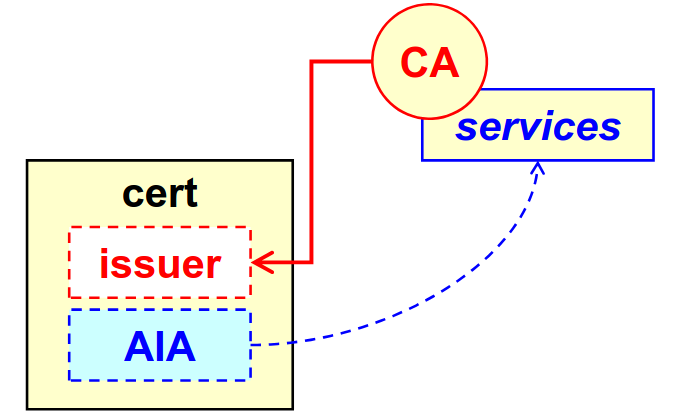
\includegraphics[width=0.5\textwidth]{img/x509 AIA.png}

  \caption{Authority Information Access (AIA) extension}
\end{figure}

\subsubsection{CA Information Access}

The \textbf{CA Information Access (CAIA)} extension serves a 
specific function in X.509 certificates, as it indicates how to 
access information and services provided by the certificate 
authority (CA) that owns the certificate. Unlike other 
extensions, CAIA is valid only within a CA certificate itself.

CAIA includes several important subfields that facilitate access 
to the CA's services, such as:
\begin{itemize}
  \item \textbf{certStatus}: This subfield may point to the status of 
    the CA's certificates, typically through an OCSP responder.
  \item \textbf{certRetrieval}: This allows for the retrieval of the 
    CA's own certificate from a designated location.
  \item \textbf{cAPolicy}: This subfield provides information on the 
    policies that govern the CA's operations, helping users 
    understand the trust model.
  \item \textbf{caCerts}: It indicates where the CA's certificates can 
    be accessed, which is vital for validating the certificate 
    chain.
\end{itemize}

The significance of CAIA lies in its role as a self-pointer for 
the CA. When you possess a CA certificate and wish to locate its 
services, CAIA provides the necessary pointers to information 
about the CA itself, including its policy, OCSP responder, and 
certificate repository. This self-referential nature distinguishes 
CAIA from other access methods, which typically point back to the 
parent CA. As with many extensions, CAIA can be classified as 
either critical or non-critical, depending on the context in 
which it is used. However, it is particularly valuable for 
establishing a complete understanding of the CA's services and 
trustworthiness.

\begin{figure}[h]
  \centering
  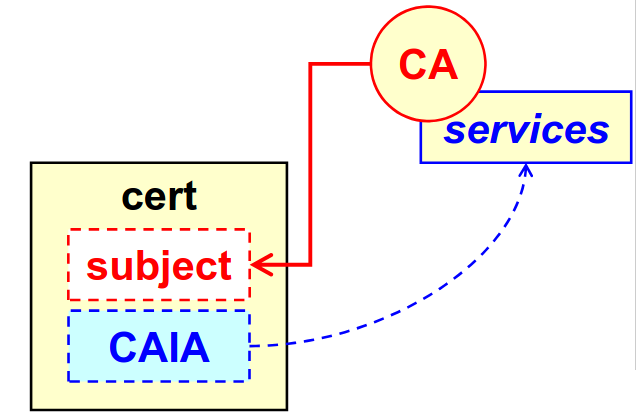
\includegraphics[width=0.5\textwidth]{img/x509 CAIA.png}

  \caption{CA Information Access (CAIA) extension}
\end{figure}

\subsubsection{RFC-2459}

The \textbf{RFC-2459} document defines a profile for the use of 
X.509v3 certificates in Internet applications, such as IPsec, TLS, 
and S/MIME. This profile was initially suggested by the Public Key 
Infrastructure (PKIX) working group to promote interoperability 
and standardization across diverse systems and protocols.

One of the key aspects of RFC-2459 is that it establishes extensions 
defined by an Object Identifier (OID), specifically using the base 
\texttt{ID-PKIX ::= 1.3.6.1.5.5.7} (which maps to 
\texttt{iso.org.dod.inet.sec.mechanisms.pkix}). OIDs ensure that 
each extension and algorithm used within the X.509 framework is 
uniquely identifiable and properly managed. For instance, PKIX 
requested an OID rooted in the U.S. Department of Defense namespace 
due to the historical origin of the internet (as DARPA Net), and 
further sub-trees were established for protocols like IPsec, TLS, 
and S/MIME.

RFC-2459 also specifies the supported algorithms that should be 
implemented to ensure secure and reliable communication. Beyond 
defining supported algorithms, it offers several implementation 
suggestions to enhance compatibility. A few examples include:
\begin{itemize}
    \item \textbf{UTC Time}: It is mandatory to include seconds 
    in time fields.
    \item \textbf{Zulu Time}: UTC time must be expressed in the 
    Zulu (Greenwich Mean Time) timezone, which avoids issues with 
    software systems that misinterpret time zones. For instance, 
    some software (notably from Microsoft) might default to local 
    time, causing inconsistencies.
    \item \textbf{Two-Digit Year Format}: Although specifying the 
    year in two digits is not recommended, when used, it should be 
    interpreted within the range of 1950-2049. After 2049, 
    certificates must switch to four-digit year formats to avoid 
    ambiguity and incompatibility issues.
\end{itemize}

By adhering to the guidelines outlined in RFC-2459, certificate 
issuers and consumers ensure proper functionality across diverse 
systems, especially in the context of internet security protocols. 
The use of standardized extensions, supported algorithms, and 
implementation details like time format further strengthens 
interoperability and the reliability of X.509 certificates.

\subsubsection{Extended Key Usage}

The \textbf{Extended Key Usage} (EKU) extension in X.509 certificates 
allows for defining specific uses of a certificate in addition to, 
or in substitution of, the standard \texttt{keyUsage} extension. 
Unlike the standard key usage, which is focused on cryptographic 
operations, EKU is oriented towards specific applications. This 
enables a certificate to be more narrowly defined for its intended 
purpose, enhancing security and clarity in certificate handling.

EKU can be used simultaneously with the standard \texttt{keyUsage} 
extension, though it is important to consider how conflicts between 
the two might be handled in practice. EKU serves to tailor 
certificates for specific tasks within certain application domains, 
which is particularly useful in environments requiring strict 
certification boundaries, such as server authentication or 
email protection.

Some of the possible values for EKU include:
\begin{itemize}
    \item \texttt{serverAuth} (\texttt{id-pkix.3.1}): This EKU 
    designates a certificate for server authentication. In cases 
    where serverAuth is used, the equivalent key usages that should 
    be enabled include Digital Signature (DS), Key Encipherment (KE), 
    and Key Agreement (KA).
    \item \texttt{clientAuth} (\texttt{id-pkix.3.2}): This EKU is 
    intended for client-side authentication and can be mapped to 
    Digital Signature (DS) and Key Agreement (KA).
    \item \texttt{codeSigning} (\texttt{id-pkix.3.3}): This EKU is 
    used for code signing, allowing developers to sign the code they 
    create. The primary associated key usage is Digital Signature 
    (DS).
    \item \texttt{emailProtection} (\texttt{id-pkix.3.4}): This EKU 
    provides a certificate for email protection. It includes Digital 
    Signature (DS), Non-Repudiation (NR), Key Encipherment (KE), and 
    Key Agreement (KA) as the relevant key usages.
    \item \texttt{timeStamping} (\texttt{id-pkix.3.8}): Used for 
    timestamping, this EKU is associated with Digital Signature (DS) 
    and Non-Repudiation (NR). Timestamping certificates are crucial 
    for certifying when a particular action, such as a signature, 
    took place.
    \item \texttt{ocspSigning} (\texttt{id-pkix.3.9}): This EKU is 
    specific to signing OCSP responses. The associated key usages 
    are Digital Signature (DS) and Non-Repudiation (NR), ensuring 
    that OCSP responses are properly authenticated.
\end{itemize}

In summary, the PKIX group developed EKU to provide more granular 
control over certificate usage within specific applications. For 
example, a certificate intended for email may only be valid for email 
protection, while another for server authentication may only serve 
that purpose. The flexibility offered by EKU allows for more precise 
security policies, tailored to the needs of individual systems or 
applications.

\subsubsection{Evolution of RFC-2459}

The evolution of \textbf{RFC-2459}, which initially defined the 
profile of X.509v3 certificates for use in Internet applications, 
reflects a series of updates and refinements to both certificate 
profiles and cryptographic algorithms.

RFC-2459 was replaced by two key documents:
\begin{itemize}
    \item \textbf{RFC-3280}: This document defines the Internet 
    profile of public key infrastructures (PKIs) based on X.509v3 
    certificates and X.509v2 certificate revocation lists (CRLs). 
    It was intended to standardize how certificates and CRLs are 
    managed and used in Internet-based PKI systems.
    \item \textbf{RFC-3279}: This document covers the algorithms 
    used in conjunction with the RFC-3280 profile, providing 
    identifiers, parameters, and encodings. It includes, and makes 
    obsolete, the earlier RFC-2528, which addressed the use of 
    the Key Exchange Algorithm (KEA).
\end{itemize}

The decision to split RFC-2459 into two separate RFCs was driven by 
the recognition that while certificate profiles tend to remain stable 
over time, cryptographic algorithms evolve more rapidly. By 
documenting algorithms separately in RFC-3279, it became easier to 
update the list of supported algorithms without needing to revise the 
entire certificate profile.

Later on, \textbf{RFC-3280} was itself obsoleted by \textbf{RFC-5280}, 
which further refined the Internet PKI profile and introduced updates 
to align with advancements in cryptographic practices and PKI 
implementation. RFC-5280 remains a foundational document in the 
definition of PKI systems used for securing Internet communication.
\subsubsection{RFC-3279 and Supported Algorithms}

\textbf{RFC-3279} specifies the algorithms that \emph{MUST} be 
supported by applications using the \textbf{RFC-3280} profile. 
It includes some older algorithms, as well as newer ones. The key 
algorithms defined in this RFC are:

\begin{itemize}
  \item \textbf{Digest algorithms:}
  \begin{itemize}
    \item MD-2, MD-5, SHA-1 (preferred)
  \end{itemize}
  \item \textbf{Algorithms for signing certificates/CRLs:}
  \begin{itemize}
    \item RSA, DSA, \underline{ECDSA (Elliptic Curve DSA)}
  \end{itemize}
  \item \textbf{Subject public key algorithms (SubjectPublicKeyInfo):}
  \begin{itemize}
    \item RSA, DSA, \underline{KEA}(a variant of Diffie-Hellman), DH
      (Diffie-Hellman), \underline{ECDSA}, \underline{ECDH (Elliptic
      Curve Diffie-Hellman)}
  \end{itemize}
\end{itemize}

The underlined algorithms were introduced in \textbf{RFC-3279} in 
comparison to \textbf{RFC-2459}. One important point is that RFC-3279 
permits the use of legacy algorithms, though they are not recommended 
(e.g., SHA-1 is preferred for digest, and RSA/DSA for certificate 
signing, with ECDSA added for more modern use). 

Once the basic definitions are set, optional algorithms can be defined. 
Notably:

\begin{itemize}
  \item \textbf{RFC-4055:} Adds better specifications for signatures, 
    including the Probabilistic Signature Scheme (PSS), Optimal 
    Asymmetric Encryption Padding (OAEP), and SHA-2 for digest 
    computation.
  \item \textbf{RFC-4491:} Addresses the needs of Russia by providing 
    specifications for the \emph{GOST} algorithm family, widely used 
    in Russian encryption standards.
  \item \textbf{RFC-5480:} Introduces elliptic curve keys of various 
    kinds.
  \item \textbf{RFC-5758:} Adds support for new algorithms in the 
    \emph{SHA-2} family, such as SHA-224 and SHA-256.
  \item \textbf{RFC-8692:} Uses SHAKE128 and SHAKE256 for signatures, 
    both part of the \emph{SHA-3} family of algorithms.
\end{itemize}

\subsubsection{RFC-3280 / RFC-5280: PKI Profile}

\textbf{RFC-3280} and \textbf{RFC-5280} specify the profile that defines 
not only values and fields but also algorithms and procedures. These 
ensure that certificates are processed consistently across the world. 
Key aspects include:

\begin{itemize}
  \item \textbf{Path validation algorithm:} Defines how to build or 
    verify the certificate chain, starting from an end entity (EE) 
    certificate, which is issued by a CA, up to a trusted root.
  \item \textbf{Certificate status verification:} Specifies details 
    for verifying the status of a certificate, using methods such as 
    the full CRL or Delta-CRL.
  \item \textbf{Extended Key Usage (EKU):} Adds the \emph{OCSPSigning} 
    extended key usage.
  \item \textbf{Certificate extensions:} Includes important extensions 
    such as:
  \begin{itemize}
    \item \textbf{Inhibit any-policy:} Prevents the use of any policy, 
      ensuring that the CA must specify its own policies.
    \item \textbf{Freshest CRL:} A pointer to a new type of CRL 
      (Delta-CRL), which contains only the differences with the last 
      full CRL.
    \item \textbf{Subject information access:} Already discussed 
      previously.
  \end{itemize}
  \item \textbf{Freshest CRL for CRLs:} If there is a Delta-CRL 
    pointer in a certificate or CRL, it is possible to access the 
    differences with the last full CRL. The Freshest CRL is also known 
    as the Delta CRL Distribution Point. It is always marked as 
    non-critical because there are multiple ways to check certificate 
    status (e.g., full CRL, Delta CRL, OCSP), and it is not feasible 
    to make any single method mandatory.
\end{itemize}

\subsubsection{Additional Points}

\begin{itemize}
  \item \textbf{Path validation focus:} Due to the sensitive nature of 
    path validation, recent RFCs have paid much more attention to 
    specifying the algorithms for this process, rather than just 
    providing high-level descriptions as in earlier versions. 
  \item \textbf{Support for internationalization:} With global use of 
    certificates, it has become important to support different 
    alphabets, such as those used in Japan, China, and India, in 
    fields like URI, DNS names, and email addresses. \textbf{RFC-8398} 
    adds support for internationalized email addresses and domain 
    names.
  \item \textbf{Freshest CRL pointer:} A crucial feature is the 
    \emph{Freshest CRL} pointer, which allows a certificate or CRL to 
    reference the latest Delta-CRL. This prevents the need to 
    redownload a full CRL when only small updates are necessary.
  \item \textbf{No Delta of Delta-CRLs:} Delta CRLs cannot be created 
    incrementally (i.e., you cannot generate a Delta of a Delta CRL). 
    Each Delta CRL must reference the base CRL directly, making the 
    process more straightforward.
\end{itemize}

\section{Certificate Revocation}

A certificate may be revoked before its natural expiration due 
to various reasons. The revocation can occur under the following 
circumstances:

\begin{itemize}
  \item \textbf{Upon request of the certificate owner (subject):}
    This typically happens due to:
    \begin{itemize}
      \item \textbf{Key compromise:} the subject knows that someone else has
        gained possession of their keys.
      \item \textbf{Key loss}: the subject cannot locate the key,
        meaning that the certificate is no longer trustworthy.
    \end{itemize}

  \item \textbf{Upon request of the certificate sponsor
    (organization):} some cases include:
    \begin{itemize}
      \item This occurs when an employee leaves the organization, 
        the company goes out of business, or a server is dismissed,
        among other reasons.
      \item Any entity no longer in use should have its certificate 
    revoked to prevent unauthorized usage.
    \item This also applies if a company shuts down or transitions 
    services, rendering previous certificates unnecessary or insecure.
  \end{itemize}
  
  \item \textbf{Autonomously by the issuer}, for a few reasons:
  \begin{itemize}
    \item \textbf{Fraud}: convinces a certification authority to issue
      a certificate based on false information. For example, a person
      could impersonate an executive or delegate to receive an
      unauthorized certificate.
    \item \textbf{Error}: because mistakes may happen sometimes
    \item In such cases, the issuer may revoke the certificate without 
    needing approval from the original certificate owner or sponsor.
  \end{itemize}
\end{itemize}

Once a certificate is revoked, it is marked as invalid, and any 
transaction using that certificate must consider it untrustworthy.

\textbf{Certificate status MUST be checked} by the entity that 
accepts the certificate to ensure that it is still valid and has 
not been revoked. This is the responsibility of the \emph{relying 
party (RP)}. 

\begin{boxH}
  The RP must always verify the certificate's status to protect any
  transaction (e.g., a commercial order) relying on the certificate
  for security.
\end{boxH}

\subsection{Mechanisms for checking certificate status}
When verifying a certificate's status, it is important to:
\begin{enumerate}
    \item Consider the entire chain of certificates up to a trusted root.
    \item Check if any certificate in the chain has expired.
    \item Ensure all certificates are valid.
    \item If a certificate has not expired, a PKC (Public Key
      Certificate) is considered valid unless otherwise stated.
\end{enumerate}

Two possible mechanisms exist to check the validity status:
\begin{itemize}
    \item \textbf{CRL (Certificate Revocation List)}, which is a list
      of revoked certificates. You check the list manually to see if a
      certificate has been revoked. The CRL is signed by the issuer or
      a delegated revocation authority.
    \item \textbf{OCSP (Online Certificate Status Protocol)} provides
      the status of a specific certificate at the current time. It
      returns an answer whether the certificate is valid at the moment
      of the request. The response is typically signed by the OCSP
      server, which may raise trust concerns.
\end{itemize}

\subsection{X.509 CRL}
The \textbf{Certificate Revocation List (CRL)} is a mechanism 
used to track revoked certificates. It contains:
\begin{itemize}
    \item A list of revoked certificates.
    \item The revocation date and reason, indicating when the 
    certificate ceased to be valid. Those details are not present 
    in the OCSP response.
\end{itemize}

CRLs are issued periodically and maintained by the certificate
issuer (CA), even if no additional revocations have occurred, a
CRL must be reissued to ensure its "freshness" and prevent replay
attacks with outdated CRLs.

RLs are digitally signed by:
\begin{itemize}
  \item The Certificate Authority (CA) that issued the 
    certificates.
  \item A revocation authority delegated by the CA. When 
    signed by the revocation authority, the CRL is referred 
    to as an \textbf{indirect CRL (iCRL)}.
\end{itemize}

For instance, at Politecnico, a CRL is generated every 30 days 
to ensure the CRL remains current, even if no new revocations 
have taken place. This practice prevents ambiguity about whether 
a CRL is outdated or if no certificates have been revoked.
\subsubsection{x.509 CRL version 2}
\begin{verbatim}
CertificateList ::= SEQUENCE {
    tbsCertList          TBSCertList,
    signatureAlgorithm   AlgorithmIdentifier,
    signatureValue       BIT STRING
}

TBSCertList ::= SEQUENCE {
    version                Version OPTIONAL,
                          -- if present, version must be v2
    signature              AlgorithmIdentifier,
    issuer                 Name,
    thisUpdate             Time,
    nextUpdate             Time OPTIONAL,
    revokedCertificates    SEQUENCE {
        userCertificate      CertificateSerialNumber,
        revocationDate       Time,
        crlEntryExtensions   Extensions OPTIONAL
    } OPTIONAL,
    crlExtensions          [0] Extensions OPTIONAL
}


\end{verbatim}
The CRL structure consists of a sequence containing the list to be
signed (\texttt{tbsCertList}), the algorithm, and the signature value.
The version field determines whether it's version 1 (if absent) or
version 2. The issuer can be the Certificate Authority (CA) or a
revocation authority. 

The \texttt{thisUpdate} field indicates the time of the latest update, 
while the optional \texttt{nextUpdate} field suggests when the next CRL 
will be created, serving as a promise to issue a new CRL by that date. 
If the next update has passed, a new CRL should be obtained.

The \texttt{revokedCertificates} field lists revoked certificates, 
providing the serial number, revocation date, and optional 
extensions. These extensions may apply to individual revoked 
certificates or to the entire CRL, and are optional in both cases.


\subsubsection{Extensions of CRLv2}
In CRLv2, there is an extension for each entry of the CRL or a global
for the whole CRL.

\begin{itemize}
    \item \textbf{crlEntryExtensions}:
    \begin{itemize}
        \item \textit{Reason Code}: Helps clarify the cause of
          revocation (e.g., key compromise vs. key destruction).
        \item \textit{Hold Instruction Code}: Marks a certificate as
          temporarily suspended, not permanently revoked. Though
          deprecated, because it forces the validators to keep a lot
          of copies just for the suspended certificates. 
        \item \textit{Invalidity Date}: Specifies when the certificate
          became invalid.
        \item \textit{Certificate Issuer}: Identifies the issuer in
          case of an indirect CRL (i.e., the CRL is signed by a
          revocation authority rather than the CA).
    \end{itemize}
    
    \item \textbf{crlExtensions}:
    \begin{itemize}
        \item \textit{Authority Key Identifier}: Supplemental
          information about the key used to sign the CRL.
        \item \textit{Issuer Alternative Name}: Provides additional
          issuer identification, supporting internet-based
          identifiers.
        \item \textit{CRL Number}: Tracks different versions of the CRL.
        \item \textit{Delta CRL Indicator}: Specifies if the CRL is a
          delta CRL (shows only differences from the base CRL). If
          it's 0 it's not a delta CRL.
        \item \textit{Issuing Distribution Point}: A pointer to the
          location where the latest CRL can be found.
    \end{itemize}
\end{itemize}

\subsubsection{Certificate revocation timeline}
A key issue arises with the \textit{revocation date}(CRLv2) and
\textit{invalidity date}(CRLv2 Extention), which are both included for
revoked certificates. Although they might seem redundant, they serve
to solve a problem.\\
Take a look at figure \ref{fig:certificate revocation timeline}, we
have a point in time (before the red part) in which everithing works
fine and the CLR number $n$ has been issued. At a certain point the
private key has been compromised, meaning that someone can impersonate
someone else. A certificate revocation in requested after the user
became aware of the issue, which would like to revoke the certificate
with a prior date or time of the one that would be issued by the CA.
Now the two dates come into play. The \textit{revocation date} is the 
date certified by the CA, while the \textit{invalidity date} is the 
date claimed by the ee.\\
The risk is not yet over, because the CA, to issue a new certificate
needs some time(the one in yellow), meaning that every request made 
in that time slot will still get the old certificate back. For this
reason any good relying party should wait to get the next issued CRL
for any important operation, while also having a strong proof of the
time when the key was used.

\begin{figure}[H]
  \centering
  \includegraphics[width=0.7\textwidth]{img/x509 certificate
  revocation timeline.png}

  \caption{Certificate revocation timeline}
  \label{fig:certificate revocation timeline}
\end{figure}
\subsubsection{Efficient management of CRLs}
The major issue with CRLs is their size. They can become quite large
over time, especially in large organizations. For this reason many
solution have been proposed.\\
One of those is to eliminate the revocation following the first CRL
issued after the expiry date of the certificate, but required an
archive in which all the past CRLs are stored.\\
Another solution is to use the \textit{Delta CRL}, by publishing the
base CRL and, from that one on, only the changes. This solution is
good for the download time, but still doesn't solve the problem of the 
storage.\\
The best solution is probably the \textbf{partitioning of the CRLs}.
For example, one CA could partiotion them in buch of 1000 certificates 
each, and to download one you need to download the whole partition.\\
In the end, a perfect solution does not exist.

\subsection{OCSP}
OCSP (as defined in RFC-6960) is an alternative to CRLs and is used to
verify if a certificate is \textbf{valid} at the \textbf{current
moment}. The protocol follows a client-server model where the server,
known as the responder, returns one of three possible responses:
\textit{good} (the certificate is valid), \textit{revoked} (the
certificate has been revoked), or \textit{unknown} (the status of the
certificate cannot be determined).

Responses from the OCSP responder are digitally signed to prevent fake
responses. Optionally, the responder may accept only signed requests
from clients to provide authentication and restrict access.  
\begin{boxH}
  Keep in mind that, because the OCSP response is signed with the
  certificate of the OCSP server, it is not possible to verify the 
  signature using OCSP itself. 
\end{boxH}

As a result, OCSP responders usually operate with short-lived
certificates, typically valid for 24 hours, requiring automation to
manage frequent certificate requests.


It is implemented as a binary protocol and does not have a 
default port. The URI, provided in the Authority Information 
Access, specifies the port on which the OCSP responder is 
available. OCSP can be encapsulated in various transport protocols 
such as HTTP, HTTPS, LDAP, and SMTP, which act as wrappers for the 
binary data exchange.

OCSP provides a real-time mechanism for checking the validity of 
certificates, but managing the responder’s certificates, especially 
with short lifetimes, often requires automation to ensure 
continuous availability and security.

\subsubsection{OCSP source of information}
OSCP, to provide an answer, must have a source of information. This
data can be aquired in different ways:
\begin{itemize}
  \item \textbf{download i form CRL repositorie}
  \item \textbf{querying the CA database}
  \item \textbf{ask another OSCP server(chaining)}
\end{itemize}
\begin{figure}[H]
  \centering
  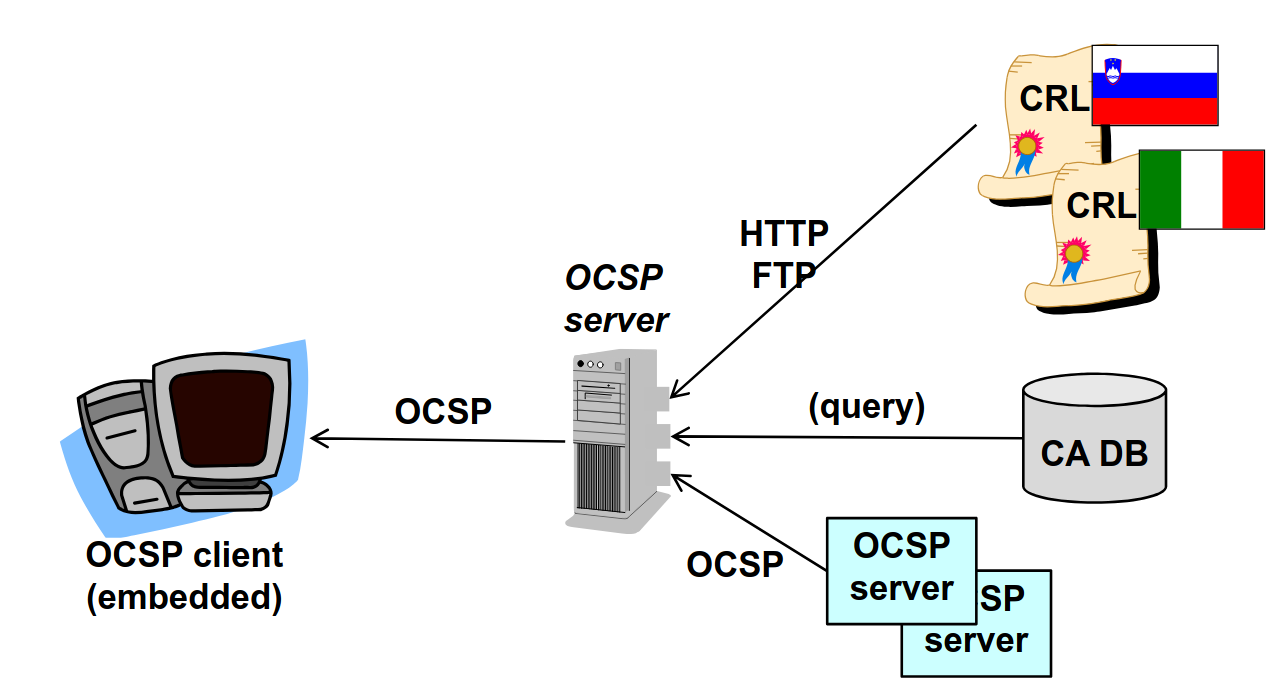
\includegraphics[width=0.5\textwidth]{img/x509 OCSP query.png}
  \label{fig:OCSP source of information}

  \caption{OCSP source of information}
\end{figure}

\subsubsection{The protocol}
Lets now go over how the protocol works.

An OCSP \textbf{request} contains three parameters:
\begin{itemize}
  \item the \textbf{protocol version}
  \item the \textbf{target certificate identifiers}
  \item the \textbf{extension}, which are optionals
\end{itemize}
In the request, each certificate is identified by its certID:
\begin{itemize}
  \item hashAlgorithm (AlgorithmIdentifier)
  \item issuerNameHash (hash of Issuer's DN)
  \item issuerKeyHash (hash of Issuer's public key)
  \item serialNumber (CertificateSerialNumber)
\end{itemize}
As you can see, in this section, no explicit information about the 
certificate is provided, and this is done for privacy reasons.

The response contains:
\begin{itemize}
    \item the version of the response syntax.
    \item the name of the responder itself.
    \item one response for each certificate in the request, allowing
      the status of multiple certificates to be requested with one
      query.
    \item the extension, optional again
    \item The OID of the signature algorithm for the signed response.
    \item The signature, which is computed across the hash of the 
          response.
\end{itemize}
The SingleResponse of each certificate contains:
\begin{itemize}
  \item The certificate identifier
  \item the certificate status, and if revoked, the revocation time
    and optionally, also the revocation reason.
  \item the thisUpdate field, which indicates the time of the response
    to indicate which is the knowledge of the responder.
  \item the nextUpdate field, which is optional
\end{itemize}

\subsubsection{Models of OCSP responder}
There are some types of models:
\begin{itemize}
  \item \textbf{CA Responder} (operated by the CA): the CA signs the
    response with its own private key, which is quite risky because
    the private key of the CA must be online, so it is rarely adopted.
    It is possible to mitigate this problem by using a key dedicated
    only to OCSP signing (remember ExtendedKeyUsage). Even if the OCSP
    responder is operated by the CA, it can use different keys: one
    for creating certificates and one to sign them. That goes also in
    the direction of “Authority Key Identifier” because a CA could
    have 3 keys: certificate sign, CRL sign, OCSP responder sign. This
    because they are different functions and maybe different machines.
    This last method is the most used one.
  \item \textbf{Trusted responder}: the OCSP server signs the
    responses with a pair key:cert independent of the CA for which it
    is responding. The company responder is something like that. It
    can be also a trusted third party (TTP) paid by the user.
  \item \textbf{Delegated responder}: the OCSP server signs the
    responses with a pair key:cert which is different based on the CA
    for which it is responding. It’s a TTP paid by the CA for who it is
    responding. An external server is delegated to provide the answer on
    the CA behalf by providing a pair key:cert where the cert contains
    OSCP responder as extended key usage, and this will show that the
    responder is delegated by the CA to provide OSCP answers. There
    could be one responder that answers for multiple CAs.
\end{itemize}
As we have seen, OSCP is faster but for real time transactions they
are quite the same. For delayed verifications we have problems because
we need to store the information at the time of the signature.
\subsubsection{Attacks against OCSP}
There are two main attacks possible against OCSP.

The first one is obviously a \textbf{replay attack}: one can ask for 
the validity of a certificate, store the response and replay it when
its not valid anymore by being faster then the OCSB server or stopping
the real response via a denial of service. For this reason, optionally
but encouraged, the client could send a
\textbf{nonce}(\texttt{id-pkix-ocsp-nonce}) in its request to the
server, which will be included in the response signed by the server.

Another possible attack is a \textbf{denial of service} one,
accomplished by flooding the OCSP server with many requests. One
little detail is esclusive of an OCSP dos attack: requests have to be
digitally signed, which takes a lot of time to verify for the server
and makes the attack easier. The obvious defence is to remove the
real-time signature and replace it with a pre-computed responses,
which requires three timestamps:
\begin{itemize}
  \item thisUpdate – the response is based on revocation information
    available now
  \item nextUpdate – is again a promise.
  \item producedAt – this answer was created in this moment.
\end{itemize}
These answers are created even if no question is made. Since we are
creating the answer without waiting for the request there is no nonce.
In order to protect from DoS attack a problem about the replay attack
is created. What some companies do is to use pre-computed responses
and try to make them fast enough (e.g, the response is valid only for
30 minutes. Again there is the need to look at the policy).

\section{Proof of possession(POP)}
One of the issues we discussed in this chapter is the fact that, in
the registration protocol that we explained, the identity of the ee is 
verified by the CA, but the CA is not sure that the private key is 
really in its possession.

\begin{boxH}
  Having a Proof of possession means that the certification authority
  has a guarantee that the private key is in possession of the subject
  requesting the certificate.
\end{boxH}
If a certification authority creates a certificate without proof of
possession, then there are various attacks possible, meaning that it
is imperative to achieve non-repudiation. On the other hand, POP is
not critical for encryption.
\subsection{Risks in the absence of POP}
Let's consider the case in which we don't have proof of possession.

Alice creates a private key and stores it locally then sends a public
key and an identifier to the CA. The CA verifies Alice’s identity and
creates a certificate associating Alice to that public key. Then
there’s Bob who sends to the same CA the same public key of Alice
(copied from another certificate) and his identifier. If the CA
doesn’t perform POP, it will create another certificate with the same
public key associated to Bob and here’s the problem. When Alice signs
a document, it may happen that when someone is contesting that
document, she could claim that Bob signed it, so there is no
non-repudiation. Another case may be that Alice claims that she signed
a document, but Bob may say it was him signing it. So, Alice can deny
a signature or Bob can claim his signature. That means that POP for
any case of non-repudiation and attribution, especially in legal
matters, is a very important thing.

\begin{figure}[H]
  \centering
  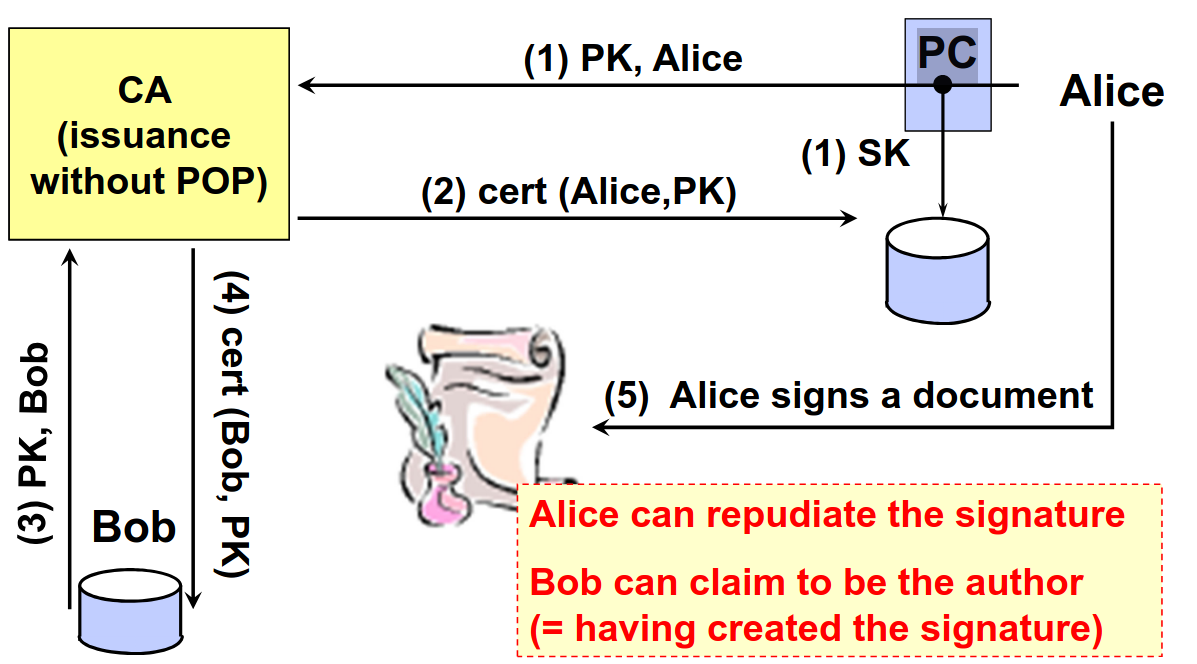
\includegraphics[width=0.6\textwidth]{img/x509 pop absence.png}
  \label{fig:risks in the absence of POP}

  \caption{Risks in the absence of POP}
\end{figure}
\subsubsection{Countermeasures}
\begin{boxH}
  The best solution to demostrate the POP is at signing time.
\end{boxH}
The signer inserts a reference to the certificate (e.g. a hash) among
the signed information, thus the signature value is a function of the
certificate too (depends on it).
Unfortunately, most of the security protocols do not perform this kind
of task. There are some custom protocols designed for protecting
electronic documents that keep this into consideration.\\

Another solution is quite simple: the CA issues a certificate only if
it has the proof that the certificate requester owns the private key.
POP with this method can be achieved in two methods:
\begin{itemize}
  \item Out-of-Band: the keys are not generated by the user, but are
    generated by the CA or the array and delivered in a secure token,
    for example a smart card. (This is what happens at politecnico).
    The possession of the token is proof enough
  \item In-Band/Online: the CA will keep a copy of all the private keys, but
    the problem is how to protect them efficiently. This is better but
    it requires a secure device or online methods. If the key is used
    for both signature and encryption, then could be possible to use
    the self-signed formats like PKCS\#10 or SPKAC.  When a request is
    performed there must be also a signature (which means using a
    private key), even if there is no certificate. the CA verifies the
    signature before creating the certificate. If on the contrary, the
    key that you are trying to certify is a purely encryption key,
    then the requester cannot sign anything because that is not a
    valid usage. In that case, you can use a challenge response
    protocol. The CA sends a challenge to the requester, sending an
    encrypted certificate with the public key of the requester. 
\end{itemize}

\section{PKCS\#10}

Focusing on PKCS10, it represents one of the most commonly used
formats today. It is specified in two RFCs: one detailing the basic
syntax, and the other focusing on its application. Despite its status
as an RFC, the format retains its original numbering and is also
referred to as a Certificate Signing Request (CSR).

A typical request includes:
\begin{itemize}
  \item The distinguished name
  \item The public key
  \item Several optional attributes
\end{itemize}

One of the notable optional attributes is the \textit{challenge
password}. This serves as a one-time password that may be provided by a
registration authority and can be utilized during both registration and
revocation processes. Revocation, in particular, involves both
administrative and technical aspects.

For instance, if a smart card is lost while in Torino, the individual
might visit the office to have their identity verified and initiate
revocation. However, if the loss occurs while abroad, such as in Japan,
physical presence at the office may not be feasible. In such
situations, an online method for initiating revocation is necessary.

While it may seem that simply making a phone call or using a website to
request revocation would be straightforward, this approach could lead
to unauthorized individuals blocking certificates. Therefore, when
submitting a revocation request online, there must be some means of
verifying that the request comes from the legitimate certificate owner.
This is often done through the use of the challenge password, providing
proof of ownership.

In addition to these elements, the request may also contain further
attributes and information pertaining to the requester.

\subsection{PKCS\#10 format}
The format of a PKCS\#10 request is shown in figure 
\ref{fig:PKCS10 structure}. The data to be certified, made up of the
DN, the public key and the optional attributes, is inserted at the
beginning of the certificiate. We know that the certificate contains a
signature generated by the private key of the requester, and this is
computed over the data to be certified. The signature is then inserted
at the end of the certificate. This is also a proof of possession.

\begin{figure}[H]
  \centering
  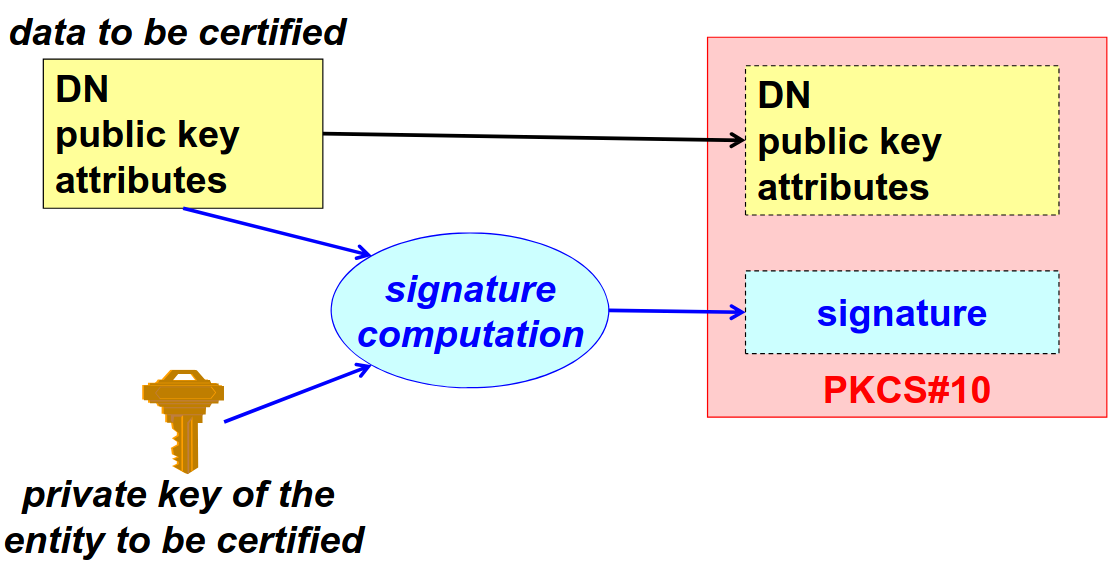
\includegraphics[width=0.6\textwidth]{img/x509 pkcs request.png}

  \caption{PKCS\#10 structure}
  \label{fig:PKCS10 structure}
\end{figure}

\subsection{Time-stamping}
In certificates, time handling is one of the most important aspects.
For that purpose we use time-stamping.
\begin{boxH}
  A time-stamp is the proof of creation of certain data
  \textbf{BEFORE} a certain point in time.
\end{boxH}
It demonstrates that data existed in that moment, but it doesn’t tell
anything about when it was created, certainly was created before but
it is not known when, and this is wrongly assumed by many people.

Time-stamping is normally performed by a \textbf{time-stamping
authority} (TSA) that uses a specific protocol and data format for its
operation. The RFC-3161 is defining the request protocol (TSP,
\textbf{Time-Stamp Protocol}) and the format of the proof (TST,
Time-Stamp Token).

\begin{figure}[H]
  \centering
  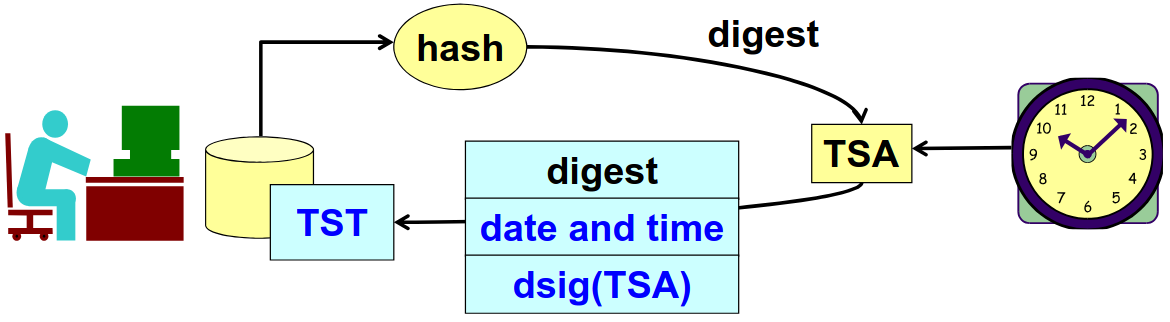
\includegraphics[width=0.6\textwidth]{img/x509 time stamping.png}
  \label{fig:time-stamping}

  \caption{the time-stamping process}
\end{figure}

The user has some data created at some point in time, which he wants
to time-stamp to demonstrate that those data existed in that moment.
The user computes a hash (it does not send data for privacy reason)
and sends it to the TSA. The authority receives the digest and
consults a very precise clock(timing is fundamental for this
procedure) and will create the TST, a document that will contain the
digest, the date and time and the digital signature of this data
performed by the time-stamping authority.

This is demonstrating that it exists in this moment, or at least that
it was created before.\\

As we just sait, the timestamp does not certify a moment in time, but
it is possible to do so with a little trick. Assume that one wants to
certify the time of a digital signature, with one timestamp $T_1$ we can
only certify that it was applied before the timestamp, but we can 
add another timestamp $T_2$ to certify that the signature was not
applied before $T_1$ to narrow the time frame, meaning that $T_2 <
\text{signature time} < T_1$. If this time frame is small enough, it
can be very accurate.

\section{Personal Security Environment (PSE)}
Let's talk for a second about something else than the public key. Most
people remember that the private key should be protected and be
secret, of course, but they forget that also the certificate of the
trusted root CA should be protected, not for confidentiality but for
authenticity. After all, a common attack is to substitute the
certificate of the trusted root CA with another one. As an additional
security features, the private key should not be exportable, meaning
that the device in which the private key is stored should be the one
used to do the operations.\\

For all those reasons, the protection mechanism are performed trough a 
\textbf{Personal Security Environment (PSE)}.

It is possible to implement PSE in software: typically it’s an
encrypted file because it contains also the private key and typically
also the root CAs. Root CAs would not require encryption but it is
done anyway since there is also the private key.

PSE can be also hardware. There are here two options: passive system
which is only a memory (like a USB pen) so it is the same as a
software PSE but hardware; active system which means that not only
protects the keys but also performs cryptographic operations using
those keys.
\subsection{Cryptographic smart-card}
Typically, the used device is a \textbf{cryptographic smart-card},
which is a chip card with memory and autonomous cryptographic
capacity. The keys need to be managed by a trusted system, if there is
an encrypted file but then the CPU is used to perform the computation
it means that the key must be put in clear in RAM for the CPU to be
used and if there’s a malware then the key could be stolen. On the
other hand, if there is a secure smart card, when the signature is
needed the CPU is sending the hash and the smart card is returning the
signature, because the smart card has the capability to perform the
computation. That is a cryptographic smart card and the difference
from a smart card for collecting points, for example, is that those
are only memory card, unlike the Polito smart card which is a
cryptographic smart-card.

These cards have microcontrollers (CPU+IO), RAM and especially an
E$^2$PROM and a cryptographic coprocessor. The E$^2$PROM is a
protected permanent memory where is typically stored the private key,
while the cryptographic coprocessor is the one that can use the key to
perform the computation. The card will never give out the key but
instead will perform the computation itself. Depending on the costs,
it is possible to have various algorithms of various lengths, the keys
can be generated on board or can be generated outside and then
injected. Typically, the memory has not lot of space. Nowadays we’re
moving from smart card to smartphones, which has both pros and cons.
The smart-card is a dedicated device that is not affected by malwares,
while smartphones are used also for other purposes and might be
affected by viruses.
\begin{figure}[H]
  \centering
  \includegraphics[width=0.6\textwidth]{img/x509 cryptographic smart
  card.png}
  \label{fig:smart-card}

  \caption{Cryptographic smart-card}
\end{figure}

A smart card is typically used by an individual and is quite slow, it
takes 1-2 seconds to perform one signature because of the small CPU
inside that works at MHz speed and because the I/O interface is
serial, one bit a time, so usually is like 9000 bits per second. This
is good to perform just a signature, but for example, a server that
needs to perform a signature needs an HSM.
\subsection{Hardware Security Module (HSM)}
A cryptographic accelerator, commonly known as a hardware security
module (HSM), provides enhanced security by offering protected memory,
where cryptographic keys are stored securely. Even if an attacker were
to access the memory, the keys cannot be extracted. In addition to
protected storage, these modules typically feature a cryptographic
coprocessor, which is responsible for performing cryptographic
operations. These are especially useful in servers for handling both
asymmetric encryption (e.g., RSA) and symmetric encryption, thanks to
their high-speed I/O capabilities.

HSMs can come in various forms, such as PCI boards, external devices
(e.g., USBI, SCSI), or network devices (e.g., netHSM). They are
essential in environments that require strong cryptographic
protections, such as electronic commerce, where TLS servers benefit
greatly from having an HSM.

\begin{figure}[H]
  \centering
  \includegraphics[width=0.6\textwidth]{img/x509 hw security
  module.png}
  \label{fig:HSM}

  \caption{Hardware Security Module (HSM)}
\end{figure}

However, integrating HSMs into cloud infrastructure presents
challenges. Cloud servers, being virtual, can be moved between
physical nodes, but HSMs are tied to specific hardware. This raises
the question of how to ensure secure key management for virtual
servers. Different cloud providers have developed various solutions,
such as virtualized HSMs, to address this issue and maintain the
necessary security level in cloud environments.
\subsection{ISO 7816-x standards for smart-card}
The ISO 7816-x standards define the physical and logical
characteristics of smart cards, there are many standars:
\begin{enumerate}
  \item Physical format
  \item Contact characteristics
  \item Electrical signals and protocols
  \item Inter-industry commands
  \item Application identifiers
  \item Inter-industry data elements
  \item SCQL (SC Query Language)
  \item Inter-industry security commands
  \item Commands for card management
  \item Electronic signals and answer to reset for sync cards
  \item Personal verification through biometric methods
  \item Cards with contacts — USB electrical interface and operating procedures
  \item Commands for application management in multi-application environment
  \item Cryptographic information application
\end{enumerate}
The most important ones are 8, 11 and 14.

\section{PKCS\#12}
If it is wanted to implement PCI in software, one of the solutions is
PKCS\#12, also called Security Bag. It is defined in RFC-7292 and it
is used to transport/store cryptographic material among different
applications and different devices in a neutral way.\\
It contains a private key and one or more certificates to transport
the digital identity of a user. It's very commonly used, for example 
by Java, Microsoft, Mozilla, Google, etc.\\ 
Beware that the extension is “.p12” but for Microsoft the files are
named “.pfx”, which has the same content with just a difference.
Microsoft has preferred speed over security, so since PKCS\#12 has a
certain number of rounds to make exhaustive attacks impossible, the
Microsoft implementation is using the lowest possible number of rounds
(more easily attackable). The suggest is to create PKCS\#12 with
another system (Mozilla, Google) and then use it on Microsoft (for
importing) but do not export from Microsoft because they will create a
lower security version of the PKCS\#12.
\begin{figure}[H]
  \centering
  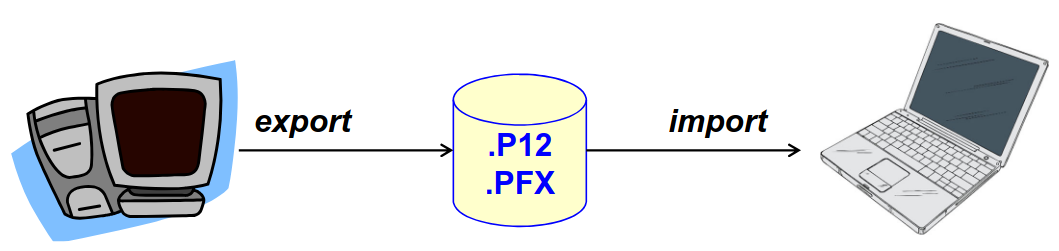
\includegraphics[width=0.6\textwidth]{img/x509 pkcs12.png}
  \label{fig:PKCS12}

  \caption{PKCS\#12}
\end{figure}


\subsection{How-to display a X.509 certificate}
The following are some useful commands to manage certificates with 
OpenSSL:

\begin{itemize}
  \item \textbf{openssl asn1parse}
    \begin{itemize}
      \item Displays the actual ASN.1 structure in abstract 
        syntax notation.
      \item May convert from the input format (PEM or DER) 
        to DER.
    \end{itemize}
  \item \textbf{openssl x509}
    \begin{itemize}
      \item Signs/verifies a certificate.
      \item The \textbf{-text} option displays the content 
        of the certificate in text format.
    \end{itemize}
  \item \textbf{dumpasn1}
    \begin{itemize}
      \item It is not part of OpenSSL but displays the content 
        of the certificate in a similar way to \textbf{asn1parse}.
    \end{itemize}
\end{itemize}

Note that when managing certificates, it is possible to have the 
ASN.1 format of the certificate stored in two different ways:

\begin{itemize}
  \item \textbf{DER} (Distinguished Encoding Rules), which is a 
    binary encoding of ASN.1 (a subset of \textbf{BER}, Basic 
    Encoding Rules).
  \item \textbf{PEM} is the armoured base64 encoding of DER.
\end{itemize}

\section{PKI organization}
PKI is a complex system that requires careful organization, in fact it
must be organized in such a way that allows for verification of the 
CRCA (Certificate Revocation Certificate Authority) trustworthiness.

\subsection{Hierarchical PKI}

A hierarchical Public Key Infrastructure (PKI) is structured as a tree
rooted at a self-signed root Certificate Authority (CA). This root CA
provides the foundation for trust within the hierarchy, but its
self-signature introduces a degree of risk due to its central role as
the root of trust.\\
One of the primary advantages of a hierarchical PKI structure is the
ease with which certification paths can be established between any two
End Entities (EEs). By traversing up the tree to a common point, a
certification path can be constructed, making this model highly
compatible with applications that natively support it. Applications
that use X.509 certificates are referred to as using PKI.\\
However, due to a range of legal, commercial, and political
challenges, there is no single global PKI hierarchy. Instead, the PKI
ecosystem is better described as a forest, with multiple independent
hierarchies or "trees." Consequently, systems often require several
root CAs, each serving as a distinct root of trust and creating its
own separate hierarchy.
\begin{figure}[H]
  \centering
  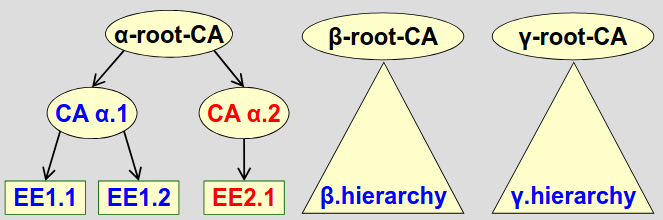
\includegraphics[width=0.6\textwidth]{img/x509 hierarchical pki.png}
  \label{fig:hierarchical PKI}

  \caption{Hierarchical PKI}
\end{figure}

\subsection{Mesh PKI}

Mesh PKI is a model designed to enable trust between entities in
different PKI hierarchies. In a standard PKI setup, different
hierarchies usually don't trust each other, which can be a hassle when
entities from one hierarchy need to communicate securely with those in
another. To solve this, Mesh PKI introduces the concept of a
\textbf{cross-certificate}, a special X.509 certificate that allows
two PKI hierarchies to trust each other either unilaterally or
bilaterally. Essentially, a root CA in one hierarchy can issue a
certificate for the root CA in another. For example, if the root of
hierarchy H3 issues a certificate for H2, then H2's root has two
certificates: one that's self-signed and another from H3. In this
case, when someone in H2 wants to be trusted by H3, they’d ideally use
the certificate issued by H3 instead of the self-signed one.\\
This setup requires applications to handle cross-certificates and pick
the right certificate chain based on who they’re communicating with.
So, if an entity in H2 knows it's sending information to someone in
H3, it can use the H3-issued certificate for smoother verification.
However, if it doesn’t know the verifier’s hierarchy, it might need to
include multiple certificates, hoping one matches the verifier’s trust
path.\\
Although Mesh PKI seems practical, it has some drawbacks. Applications
generally don’t recognize cross-certificates automatically, so they
may struggle to pick the correct chain. Plus, if there are a lot of
hierarchies, achieving universal trust would require a ton of
cross-certificates—about \(\frac{N(N-1)}{2}\), where \(N\) is the
number of hierarchies. Due to these limitations, especially in
applications, Mesh PKI is mostly theoretical and isn’t widely used.

\begin{figure}[H]
  \centering
  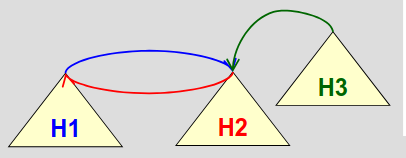
\includegraphics[width=0.5\textwidth]{img/x509 mesh pki.png}
  \label{fig:mesh PKI}

  \caption{Mesh PKI}
\end{figure}

\subsection{Bridge PKI}

In certain sectors, some organizations have opted for the bridge PKI
model over a traditional forest of hierarchies. The bridge PKI
approach introduces a special entity called the "bridge CA," which
serves as a central hub to simplify management tasks—such as adding or
removing a CA—and streamline trust transitivity across organizations.
In this model, the bridge CA is trusted by all the root CAs and
establishes cross-certification with each one. Importantly, the bridge
CA doesn’t certify any other CA or EE; it only manages
trust relationships between root CAs.\\
Adding a new CA in this model is straightforward: only two
certificates are needed, one issued by the bridge CA for the new CA
(e.g., H3) and another by the new CA for the bridge. This arrangement
enables bidirectional trust, allowing all users within the network to
reach any other user. However, like with mesh PKI, standard
applications often don’t recognize the bridge PKI model automatically,
so modifications to applications may be required to manage these
cross-certifications.\\
A prominent example of bridge PKI in practice is the U.S. Federal PKI.
In this setup, each department or local government manages its own
hierarchy, and a federal bridge CA issues the necessary
cross-certificates to link them. Additionally, some browsers, such as
modified versions of Chrome and Edge, support this model to enable
compatibility with the federal PKI. You can learn more about it at
\url{https://fpki.idmanagement.gov/}.

\begin{figure}[H]
  \centering
  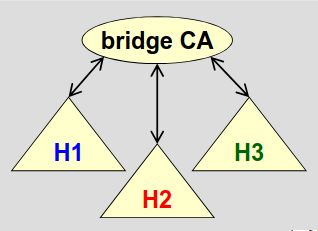
\includegraphics[width=0.3\textwidth]{img/x509 bridge pki.png}
  \label{fig:bridge PKI}

  \caption{Bridge PKI}
\end{figure}

\section*{Handling Public Key Certificates Issued Mistakenly or by
Compromised CAs}

Detecting fraudulently issued certificates for a domain is challenging
for domain owners. Imagine managing servers for an institution like
Politecnico di Torino. Under normal circumstances, a valid certificate
ensures secure communication. However, if an attacker manages to
obtain a certificate for this domain from a different CA, and this in
some instances is unexpectdly easy ( think about the Common Law and
its trust system), this fraudulent certificate would still appear
legitimate, as no notification mechanism exists to alert the domain
owner of unauthorized certificate issuance. This poses a risk, as
clients connecting to a compromised or fake server using this
certificate would see it as trustworthy. \\
Browsers are also not well-equipped to detect these malicious
certificates in real-time. Specifically, in a TLS connection, a
browser may not flag:
\begin{itemize}
    \item Certificates mistakenly issued to an unauthorized entity
    \item Certificates issued by a compromised CA
\end{itemize}

When such certificates are detected, revocation is required to alert
browsers. However, this process takes time, leaving a window during
which a browser may continue to trust a compromised certificate. This
vulnerability can lead to severe attacks, such as:
\begin{itemize}
    \item Connections to a fake server masquerading as the legitimate
      site
    \item Man-in-the-middle (MITM) attacks, where an attacker
      intercepts and manipulates data in transit
\end{itemize}

\subsection*{Some examples of mistakenly issued certificates}

Instances of mistakenly issued certificates highlight the risks of
unauthorized certificate issuance by certificate authorities (CAs).
Notable cases include:

\begin{enumerate}
  \item \textbf{2011: DigiNotar Incident} \\
    In July 2011, an intruder acquired a valid certificate for the domain \texttt{google.com} and its subdomains from the prominent Dutch Certificate Authority DigiNotar. This certificate may have been used maliciously for weeks before its detection on August 28, 2011, enabling large-scale MITM attacks against users in Iran. Some suspect the involvement of state actors aiming to spy on users of Google services. By setting up a fake website, attackers could intercept traffic to legitimate Google servers, facilitating covert surveillance.

  \item \textbf{2011: Comodo Group Incident} \\
    Also in 2011, the Comodo Group suffered a security breach that resulted in the issuance of nine fraudulent certificates for domains owned by Google, Yahoo!, Skype, and others. This attack underscored the vulnerability of even well-established CAs to unauthorized certificate issuance.

  \item \textbf{2014: India CCA Incident} \\
    In July 2014, a sub-CA of India CCA, specifically the Indian NIC (Network Information Center), misissued a substantial number of certificates. Given the incident's scope, with numerous unauthorized certificates generated, the sub-CA was fully revoked. Additionally, India CCA was restricted to issuing certificates solely for specific domains within India’s namespace. For example, it could no longer issue certificates for general domains ending in ``.in'' but only for designated domains within that scope.
\end{enumerate}

\section{HTTP Key Pinning (HPKP)}

HTTP Key Pinning (HPKP) is a security feature designed to protect
HTTPS websites from impersonation attacks by modifying the HTTP
protocol. In this approach, a site specifies the digest of its own
public key and/or one or more Certificate Authorities (CAs) in its
chain, excluding the root CA.\\
When a user agent (UA), typically a browser or an application,
accesses the site, it caches the specified key(s) and subsequently
refuses to connect to the site if it presents a different key. This
mechanism employs a Trust On First Use (TOFU) technique, meaning that
trust is established during the initial connection. However, if the
first connection is made to a fake site, the UA may refuse to connect
to the legitimate site afterward.

While HPKP provides some protection, it also poses several risks and
challenges:

\begin{itemize}
  \item Losing control of the key can lead to significant security
    vulnerabilities. For instance, if a hardware security module
    (HSM) is broken and the old private key is lost, no one will
    trust the new private key.
  \item Key updates can be problematic, especially if keys are
    changed periodically. If the current key is lost without a
    backup, it can lock users out from connecting to the server.
  \item To mitigate these risks, it's advisable to always include at
    least two keys: the current key and a backup key that is already
    provided for future use.
  \item A URI for reporting violations can be specified, allowing
    the site to operate in either enforcement mode (reporting
    refused connections) or report-only mode (notifying about
    connections to servers with different keys).
\end{itemize}

The primary purpose of HPKP is to protect against fake websites
attempting to impersonate legitimate sites using fraudulently obtained
public key certificates (PKCs). However, due to its limitations and
potential risks, HPKP has been deprecated in favor of Certificate
Transparency, which offers a more robust mechanism for monitoring and
validating the authenticity of certificates.

\section{Certificate Transparency (CT)}

Certificate Transparency (CT) is an open, global auditing and
monitoring system designed to enhance the security of digital
certificates. More information can be found at
\url{https://www.certificate-transparency.org/}. CT is based on a
public log of issued certificates, allowing domain owners, such as
Politecnico Torino, to verify that no fraudulent certificates have
been issued for their domains.

In the past, certificates issued were only visible by scanning various
repositories. Now, with CT, there is a publicly available log that
enables domain owners to scan and check if any certificates have been
issued for their domain. This transparency helps prevent issues
arising from maliciously issued certificates.

Originally proposed by Google, CT was later standardized by the IETF
Public Notary Transparency Working Group. Key features of Certificate
Transparency include:

\begin{itemize}
    \item The issuance and existence of TLS certificates are made open
      to analysis by domain owners, Certificate Authorities (CAs), and
      domain users.
    \item Web clients, including browsers and apps, should only accept
      certificates that are publicly logged in CT.
    \item It should be impossible for a CA to issue a certificate for
      a domain without it being publicly visible in the CT logs.
\end{itemize}

Implementing Certificate Transparency requires modifications in both
browsers and apps. When a web client receives a certificate, it must:

\begin{itemize}
    \item Cryptographically validate the certificate chain.
    \item Check the revocation status for each element in the chain.
    \item Verify that the certificate is present in the public log.
\end{itemize}

These requirements necessitate changes in the issuance procedures of
CAs to ensure that no certificate can be issued without being logged
publicly, thereby mitigating the risk of fraudulent certificate
issuance and enhancing overall web security.

\begin{boxH}
  The main idea of certificate transparence is to make impossible (or
  at least very difficult) for a CA to issue a PKC for a domain
  without making it visible to the domain owner.
\end{boxH}
It also aims provide an external system to the CA that lets any domain
owner or CA determine if these fraudulent certificates have been
created while also protecting the users from being given fraudulent 
certificates.

\subsection{CT – Log Servers}
Log servers are the core of the Certificate Transparency (CT) system.
They play a crucial role in maintaining a secure log of TLS
certificates. Key characteristics of log servers include:

\begin{itemize}
    \item \textbf{Append-only}: Certificates can only be added to a
      log; they cannot be deleted, modified, or retroactively
      inserted. This design ensures the integrity of the log.
    \item \textbf{Cryptographically assured}: Log servers utilize
      cryptographic techniques to ensure that the logs are
      tamper-proof.
    \item \textbf{Merkle Tree Hashes}: These hashes are employed to
      prevent tampering and misbehavior within the log, providing a
      structured way to verify the integrity of the data.
    \item \textbf{Publicly auditable}: Anyone can query a log using
      HTTPS GET and POST requests. This feature allows users to verify
      that the log is functioning correctly and to check that a
      specific TLS certificate has been legitimately appended to it.
\end{itemize}
\subsubsection{CT – Log Signature and Support}

Log entries must be digitally signed to ensure their integrity and
authenticity. The specifications for log signatures include:

\begin{itemize}
  \item \textbf{Signature Algorithms:}
    \begin{itemize}
      \item For version 1.0: NIST P-256 or RSA-2048
      \item For version 2.0: NIST P-256, Deterministic ECDSA, or
        Ed25519
    \end{itemize}

  \item \textbf{Deterministic ECDSA:} 
    \begin{itemize}
      \item Based on RFC-6979, titled “Deterministic Usage of the DSA
        and ECDSA.”
      \item If the $K$ value used in the computation is not random,
        the secret key ($SK$) can be computed from the signature,
        which poses a problem particularly in embedded systems.
    \end{itemize}

  \item \textbf{CT Support in Browsers:}
    \begin{itemize}
      \item In Chrome/Chromium/Safari:
        \begin{itemize}
          \item 1 Signed Certificate Timestamp (SCT) from a currently
            approved log.
          \item Duration $<$ 180 days: Requires 2 SCTs from
            once-approved logs.
          \item Duration $>$ 180 days: Requires 3 SCTs from
            once-approved logs.
        \end{itemize}
      \item In Firefox: CT support is pending implementation.
    \end{itemize}
\end{itemize}

\subsection{CT – Operations}

In the Certificate Transparency (CT) system, anyone can submit a
certificate to a log server, although most submissions will typically
come from Certificate Authorities (CAs) and server operators. Upon
submission, the logger provides each submitter with a commitment to
log the certificate within a specified time frame. This commitment is
known as a Signed Certificate Timestamp (SCT), which accompanies the
certificate throughout its lifetime, ensuring ongoing verification.

The SCT, created by the log servers, is delivered alongside the
certificate issued by the CA through various mechanisms. One common
method is using an X.509v3 extension to include the SCT directly in
the certificate. Alternatively, the SCT can be integrated as a TLS
extension during the handshake process, or it can be stapled to the
OCSP response, providing real-time validation of the certificate's
status.

\subsubsection{SCT via X.509v3 extension}
Before issuing a certificate, the CA contacts the Log servers and sends a
pre-certificate to it. Log server accepts the pre-certificate and returns the
SCT by logging that the CA promised to issue a certificate for a web server.
The SCT is ready, then the CA will attach the SCT to the pre-certificate as
an X.509v3 extension, then it is signed and sent to the web server. From
this moment, the web server when performing the TLS handshake will
send its certificate together with the SCT. That means that the browser does
not have to look for the SCT.
\subsubsection{SCT via TLS extension}
In this situation, CA issues a normal certificate to the server, and
server operator (the owner of a website) submit it to the log server.
Log server sends the SCT directly to the server operator and now the
web server can deliver it to the client, this time separately, using the
\texttt{signed\_certificate\_timestamp} TLS extension and it is delivered
during the TLS handshake.
\subsubsection{SCT via OCSP Stapling}
In this case, the CA informs the Log server of the creation of the
certificate and will get the log response, but this SCT is not part of
the certificate, since it has already been issued to the web server.
When the website will perform OCSP stapling (when it will require
an OCSP response from the CA) the OCSP response from the CA will
contain also the SCT. Now, the SCT will be transmitted to the
browser as part of the OCSP response.
They are different strategies that depend on the specific situation.
There is no reason to use the TLS approach if the CAs is providing
the service, for instance.

% 3 subfigures in a row 
\begin{figure}[H]
  \centering
  \begin{subfigure}[b]{0.2\textwidth}
    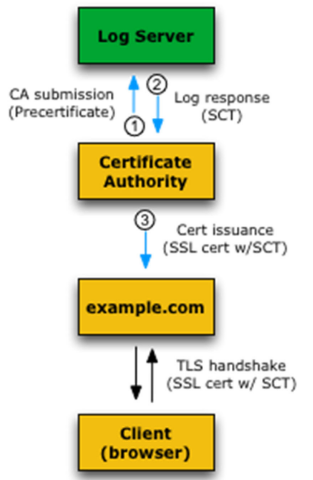
\includegraphics[width=\textwidth]{img/x509 stc v3.png}
    \caption{SCT via X.509v3 extension}
    \label{fig:ct x509}
  \end{subfigure}
  \hfill
  \begin{subfigure}[b]{0.3\textwidth}
    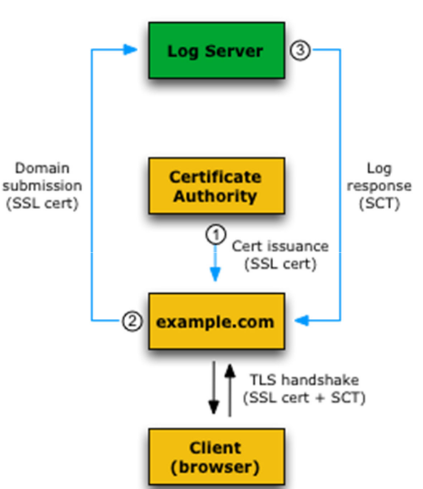
\includegraphics[width=\textwidth]{img/x509 sct tls.png}
    \caption{SCT via TLS extension}
    \label{fig:ct tls}
  \end{subfigure}
  \hfill
  \begin{subfigure}[b]{0.3\textwidth}
    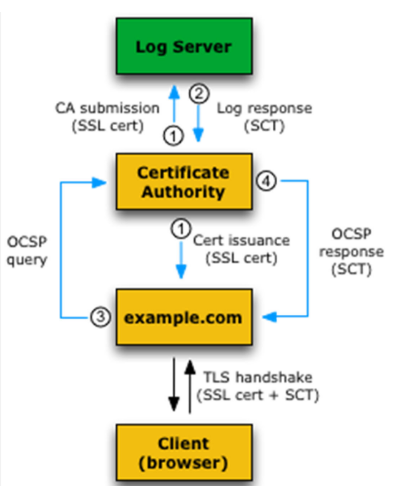
\includegraphics[width=\textwidth]{img/x509 sct oscp.png}
    \caption{SCT via OCSP Stapling}
    \label{fig:ct ocsp}
  \end{subfigure}
  \caption{SCT delivery methods}
  \label{fig:ct delivery}
\end{figure}

\subsection{Submitter and Monitors}

In the Certificate Transparency (CT) ecosystem, submitters are
responsible for submitting certificates, or partially completed
certificates, to a log server, after which they receive a Signed
Certificate Timestamp (SCT). This SCT serves as proof that the
certificate has been logged. 

On the other hand, Certificate Monitors, which are public or private
services, play a critical role in maintaining the integrity of the
system. These monitors, not previously detailed in the schemas we've
discussed, actively watch for misbehaving logs or suspicious
certificates. They periodically contact log servers to download the
latest information and inspect new entries. Additionally, they
maintain copies of the entire log and verify the consistency between
the published revisions of the log. This vigilant monitoring helps
identify potential issues, ensuring trust in the certificate issuance
process.

\subsection{ Submitter and Monitors}

In the Certificate Transparency framework, submitters play a crucial
role by submitting certificates, or partially completed certificates,
to a log server in exchange for a Signed Certificate Timestamp (SCT).
This SCT serves as proof that the certificate has been logged
properly.

Certificate Monitors, which may be public or private services, are
responsible for ensuring the integrity of the system. These monitors
actively watch for misbehaving logs or suspicious certificates. They
periodically contact log servers to download the latest information
and inspect new entries, while maintaining copies of the entire log.
They verify the consistency between published revisions of the log.

Auditors in this context are typically lightweight software components
rather than individuals. They function by verifying the overall
integrity of the logs, periodically checking log proofs. A log proof
consists of a signed cryptographic hash of the log, ensuring that a
particular certificate appears in the log. This is essential since the
CT framework mandates that all certificates must be registered; a
certificate that hasn't been registered is deemed suspect. 

While TLS clients are not required to enforce certificate
transparency, it is advisable for them to provide warnings when
connecting to a site lacking transparency. For instance, a warning
might state, "Beware, you are connecting to a website that cannot
provide certificate transparency. Do you want to proceed?" If a TLS
client, through an auditor, determines that a certificate is absent
from the log, it can use the SCT from the log as evidence that the log
has not behaved correctly. Furthermore, auditors and monitors exchange
information about logs through a specific protocol known as a gossip
protocol.

\subsection{A Possible CT System Configuration}

A Certificate Transparency (CT) system can be configured in various
ways, but a possible configuration includes the following components:

\begin{itemize}
    \item[(A)] Monitors continuously observe logs for suspicious
      certificates and verify that all logged certificates are
      publicly visible.
    \item[(B)] Certificate owners can query these monitors to ensure
      that no illegitimate certificates have been logged for their
      domain.
    \item[(C)] Auditors are responsible for verifying that the logs
      are functioning correctly and can also confirm that a particular
      certificate has been logged.
    \item[(D)] Monitors and auditors exchange information about logs
      to detect any forked or branched logs, ensuring consistency
      within the system.
\end{itemize}

\begin{wrapfigure}{r}{0.4\textwidth}
  \centering
  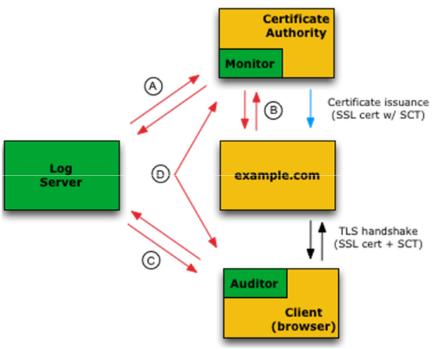
\includegraphics[width=0.4\textwidth]{img/x509 ct system.png}
  \label{fig:ct system}

  % \caption{CT System Configuration}
\end{wrapfigure}

While CT does not prescribe any specific configuration, a possible
setup might involve the following steps:
\begin{enumerate}
  \item The Certificate Authority (CA) obtains an SCT from a log
    server and incorporates it into the TLS certificate using an
    X.509v3 extension.
  \item The CA then issues the certificate, with the SCT attached, to
    the server.
  \item During the TLS handshake, the TLS client receives the TLS
    certificate along with the SCT.
  \item The TLS client validates the certificate and checks the log
    signature on the SCT to confirm that the SCT was issued by a
    legitimate log and corresponds to that certificate. If any
    discrepancies are found, the TLS client may reject the
    certificate.
\end{enumerate}

In another configuration, monitors may be operated by the CA, while
auditors can be built directly into the browser. In this case, the
browser periodically sends a batch of SCTs to its integrated auditing
component, requesting verification of whether these SCTs have been
legitimately added to a log. Auditors then asynchronously contact the
logs to perform the necessary verification.

Overall, monitors and auditors can operate as standalone entities,
offering either paid or unpaid services to CAs and server operators.

\begin{wrapfigure}{r}{0.4\textwidth}
  \centering
  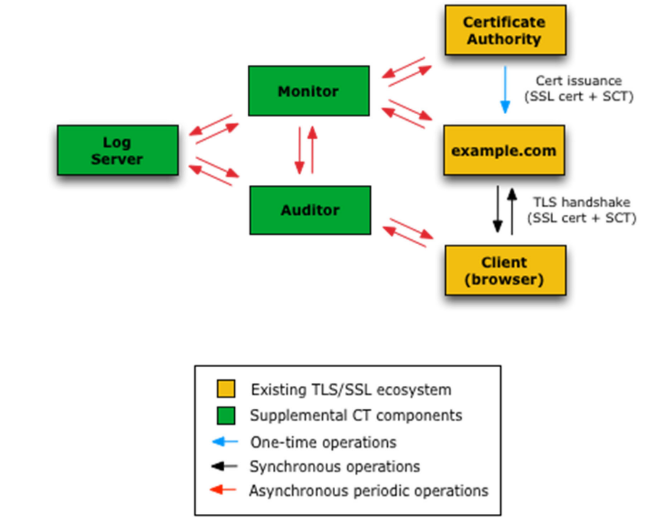
\includegraphics[width=0.4\textwidth]{img/x509 ct system alt.png}
  \caption{CT System Configuration}
  \label{fig:ct system alt}

\end{wrapfigure}

Another possible configuration is shown in figure \ref{fig:ct system
alt} , and involves placing the monitor and auditor outside the
Certification Authority  and the browser. In the previous setup, these
components were integrated within the CA and the browser, which
necessitates certain changes. However, this is not mandatory. By
having the monitor and auditor operate as independent entities, we can
minimize modifications to the existing certification authorities and
browsers.

\subsection{Current Log Servers}

As of October 2023, the availability of log servers in the Certificate
Transparency (CT) ecosystem is dependent on browser support. There are
currently six valid log servers: CloudFlare, DigiCert, Google, Let’s
Encrypt, Sectigo, and TrustAsia. For a complete list, visit
\url{https://certificate.transparency.dev/logs/}.

Additionally, there are ten public monitors that actively observe
these logs: Censys, CloudFlare, crt.sh (by Sectigo), DigiCert,
Entrust, Facebook, KEYTOS, Hardenize, sslmate, and ReportURI. It is
worth noting that many of these monitors focus primarily on the
domains they serve, such as CloudFlare, which monitors only its own
domains. For more information on public monitors, refer to
\url{https://certificate.transparency.dev/monitors/}.

\section{ACME Protocol}

The Automated Certificate Management Environment (ACME) protocol,
detailed in RFC-8555 from March 2019, simplifies the management of
public key certificates (PKCs) between End Entities (EEs) and
Certificate Authorities (CAs). Created by the Internet Security
Research Group (ISRG) for their CA service, Let’s Encrypt
(\url{https://letsencrypt.org}), ACME aims to make it easier for
everyone to adopt Transport Layer Security (TLS) without the cost.

One major challenge in the world of certificates is the push for
short-lived ones. Imagine needing to create a new certificate every 24
hours or even more frequently—that sounds like a nightmare if done
manually! This is where automation comes into play. With ACME, you can
automatically request and issue PKCs without needing a person to
intervene each time. This is especially useful since some folks
advocate for certificates valid for as little as five minutes. If a
key gets compromised, the risk is limited because the certificate
isn’t valid for long.

Here’s how it works: an ACME agent (or client) is installed on your
web server. This client proves to the CA (Let’s Encrypt) that it
controls a domain. Once the CA verifies this, it allows the client to
request and install certificates as needed. The client can even be
programmed to perform certificate operations at fixed intervals—no
more manually generating individual PKCS\#10 requests or proving domain
ownership every single time. You can also skip the hassle of
downloading and configuring server certificates with ad-hoc
procedures.

There are over 100 open-source ACME clients available, making it very 
easy to integrate this process into your workflow. Some popular ones
include Certbot (from Let’s Encrypt), GetSSL, Posh-ACME, Caddy, and
ACMESharp. For a full list, check out
\url{https://letsencrypt.org/docs/client-options/}.

By minimizing human involvement and keeping costs low, Let’s Encrypt
makes it possible for anyone to get free certificates, helping to
spread TLS adoption far and wide. With ACME handling the heavy
lifting, securing your web presence has never been easier!

If you want to use ACME for your own certificates, first of all, you
must create an account at Let's Encrypt or the CA that supports ACME.
Then you must perform domain validation once and for all, by
demonstrating that you have the right to request certificate for
a domain website. And then you will get a certificate and you will be able
also to manage the revocation of certificates.

\subsection{Account Creation}

Account creation in the ACME system is a one-time process that must be
completed before you can issue or revoke any certificates. During this
phase, the ACME client generates an asymmetric key pair, which is used
for both authentication and authorization purposes, although it's
referred to as the authorized key pair.

The authorized public key is linked to the account registered at Let’s
Encrypt, while the authorized private key is used to sign your
certificate requests. When you send a request to Let’s Encrypt,
they'll validate it using your public key. 

It's important to note that a single account can be associated with
one or more domains. While you only need one domain to start, you can
also manage certificates for additional domains, such as those
belonging to the University of Torino, under the same account.

\subsection{Domain Validation}

Domain validation is the trickiest part of the ACME protocol because
the client must prove control over the domain without human
intervention. For example, if the client claims ownership of
\texttt{Polito.IT}, the Certificate Authority (CA) will issue a
challenge. The CA might say, "If you control \texttt{Polito.IT},
please place this value in a specific path on your web server,"
meaning the client must create a web page with that value.
Alternatively, the client can create a DNS record with the value,
providing two options for validation.

In addition to placing the value, the client needs to sign a nonce
with its authorized private key to associate the proof. After the
client solves the challenge, it sends the signed nonce to the CA to
initiate the validation process. The CA then downloads the response
from the domain and verifies both the correctness and the signature.

If everything checks out, the CA approves the domain ownership by
recording it in a database, enabling the client to request
certificates for that domain. For instance, if the client claims
control of \texttt{example.com}, Let's Encrypt might challenge,
"Please place the value \texttt{ED98} on the page at
\texttt{https://example.com/80303}." The page should contain only that
value.

The client, using its private key, signs the nonce and sends it
alongside the value to the CA. Once the administrator places
\texttt{ED98} on the specified page, Let's Encrypt verifies the
response. This process links the client's public key to
\texttt{example.com} in the CA's database, allowing it to make future
requests for certificates. Notably, the private key used to sign the
message is that of the client software, not the web server. The client
acts like a chatbot, managing certificate requests for domains it
controls, such as \texttt{example.com}.

\begin{figure}[H]
  \centering
  \includegraphics[width=0.6\textwidth]{img/ACME domain
  validation.png}
  \label{fig:acme}

  \caption{ACME Domain Validation}
\end{figure}

\subsection{Certificate Request and Issuing}

Once the ACME client has been registered, it can use the authorized
key pair to request, renew, and revoke certificates for its domain.
The client constructs a PKCS\#10 Certificate Signing Request (CSR)
automatically, so there's no need for manual intervention. It submits
this request to the Certificate Authority (CA) to issue a certificate
containing a specified public key. 

In this process, the client takes the public key for a server and
includes it in the CSR. The CSR includes a signature generated by the
private key (SK) corresponding to the public key (PK) included in the
CSR. Essentially, this means the request is double-signed: it is
signed by the server’s private key and also signed with the authorized
private key associated with the domain. 

For example, when requesting a certificate for \texttt{example.com},
the PKCS\#10 structure remains unchanged, but the request is validated
by the client’s authorized key, demonstrating that it is a legitimate
request. Once the CA (e.g., Let’s Encrypt) verifies the request, it
will return a signed certificate for \texttt{example.com} that
corresponds to the specified public key, completing the issuance
process.

\begin{figure}[H]
  \centering
  \includegraphics[width=0.6\textwidth]{img/ACME certificate request
  and issuing.png}
  \label{fig:acme cert}

  \caption{ACME Certificate Request and Issuing}
\end{figure}

\subsection{Certificate Revocation}

For certificate revocation, it is the ACME client, not the server,
that signs a revocation request using the authorized private key (SK)
associated with the corresponding domain. This ensures that the client
has the right to initiate the revocation process. The Certificate
Authority verifies the signature of the request to confirm the
authorization.

Once verified, the CA revokes the specified certificate, which was
initially issued by the CA. This revocation information is then
included in the appropriate revocation mechanisms, such as the
Certificate Revocation List and/or the OCSP. Consequently, when
relying parties check the status of the certificate, they will receive
accurate and up-to-date information regarding its validity. The use of
the authorized key for this request is crucial, as it demonstrates the
client's entitlement to perform the operation, ensuring that the
revocation process is secure and properly managed.

\begin{figure}[H]
  \centering
  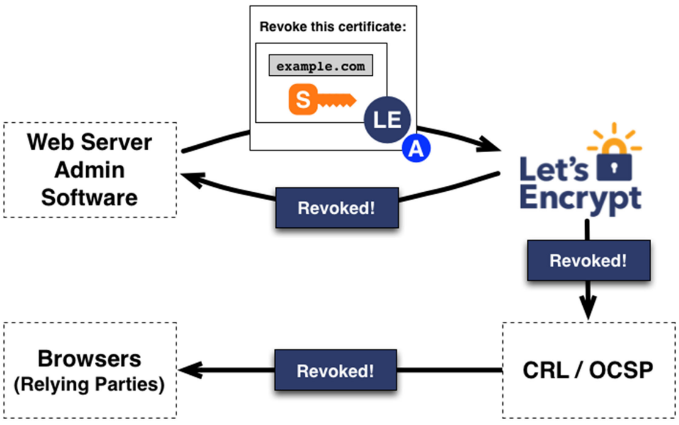
\includegraphics[width=0.6\textwidth]{img/ACME certificate revocation.png}
  \label{fig:acme rev}

  \caption{ACME Certificate Revocation}
\end{figure}
